% E02. Calidad y cobertura de la informacion.
% Va en el dossier en lugar de la seccion E02 de la plantilla:
%   % E02. Calidad y cobertura de la informacion.
% Va en el dossier en lugar de la seccion E02 de la plantilla:
%   % E02. Calidad y cobertura de la informacion.
% Va en el dossier en lugar de la seccion E02 de la plantilla:
%   % E02. Calidad y cobertura de la informacion.
% Va en el dossier en lugar de la seccion E02 de la plantilla:
%   \input{evidencias/E02_calidad_cobertura}
% Para que los pies digan "Tabla" y no "Cuadro", el preambulo del dossier
% debe decir \PassOptionsToPackage{spanish,es-tabla}{babel}.
% Cifras: 03_outputs/tables/05_resumen_calidad_E02.csv, 04_control_calidad_clima.csv,
% 04_PET_resumen_vs_CAMELS.csv, 04_PET_mensual_vs_CAMELS.csv, 05_pettitt_clima_anual.csv
% y 05_estacionariedad_clima_anual.csv,
% todas generadas por run_all.R.
% Periodo 1987-2019: acordado por el equipo el 19-oct (periodo_inicio y
% periodo_fin en 06_config).
% Fuente del caudal: Mapas DGA, reporte Caudal Diario Historico (fila Q_DGA de data_sources).
% Serie de caudal usada: la rellenada por Alexis (caudal_diario_para_airGR_1987_2019.csv),
% decidido por el equipo el 19-oct.
% Poligono: el de Alexis (cuenca_rio_damas.gpkg), desde el 19-oct.

\section{E02. Calidad y cobertura de la información}
\label{ev:E02}

\campo{1. Pregunta o afirmación que se evalúa}{¿Son suficientes y
consistentes la precipitación, las temperaturas, la PET y el caudal para
compararlos año a año en el período de análisis 1987--2019?}

\campo{2. Evidencia principal}{La Tabla~\ref{tab:E02cobertura} resume la
fuente, el registro y la cobertura de cada variable, y la
Figura~\ref{fig:E02faltantes} muestra dónde están los días sin caudal. La
Tabla~\ref{tab:E02controles} reúne los controles y las comparaciones con
otras fuentes. Las Tablas~\ref{tab:E02pettitt} y~\ref{tab:E02estacionariedad}
muestran las pruebas de homogeneidad y estacionariedad de las series anuales
del clima. La Figura~\ref{fig:E02pet} compara el ciclo
anual de la PET calculada con el de CAMELS-CL.}

\begin{table}[ht]
\centering
\caption{Fuente, registro y cobertura por variable. Cobertura: porcentaje de
días con dato dentro de 1987--2019.}
\label{tab:E02cobertura}
\begin{tabular}{|p{0.17\linewidth}|p{0.32\linewidth}|p{0.17\linewidth}|p{0.16\linewidth}|}
\hline
Variable (unidad) & Fuente & Registro & Cobertura 1987--2019, en \% \\
\hline
P (mm\,día$^{-1}$) & CR2MET v2.5 \citep{Boisier2023} & 1960-01-01 a 2021-12-31 & 100 \\
\hline
Tmax, Tmin (°C) & CR2MET v2.5 \citep{Boisier2023} & 1960-01-01 a 2021-12-31 & 100 \\
\hline
Tmed (°C) & (Tmax + Tmin)/2 & 1960-01-01 a 2021-12-31 & 100 \\
\hline
PET (mm\,día$^{-1}$) & \citet{Hargreaves1985} con Tmax y Tmin de CR2MET v2.5 & 1960-01-01 a 2021-12-31 & 100 \\
\hline
Q (m$^3$\,s$^{-1}$) & DGA, estación Río Damas en Tacamo \citep{DGA_mapas}, rellenada por el integrante 2 & 1986-02-01 a 2026-06-15 & 97.12 observado (347 días sin dato); 100 con el relleno \\
\hline
\end{tabular}
\end{table}

\begin{figure}[ht]
\centering
\IfFileExists{../03_outputs/figures/05_cobertura_caudal.png}{%
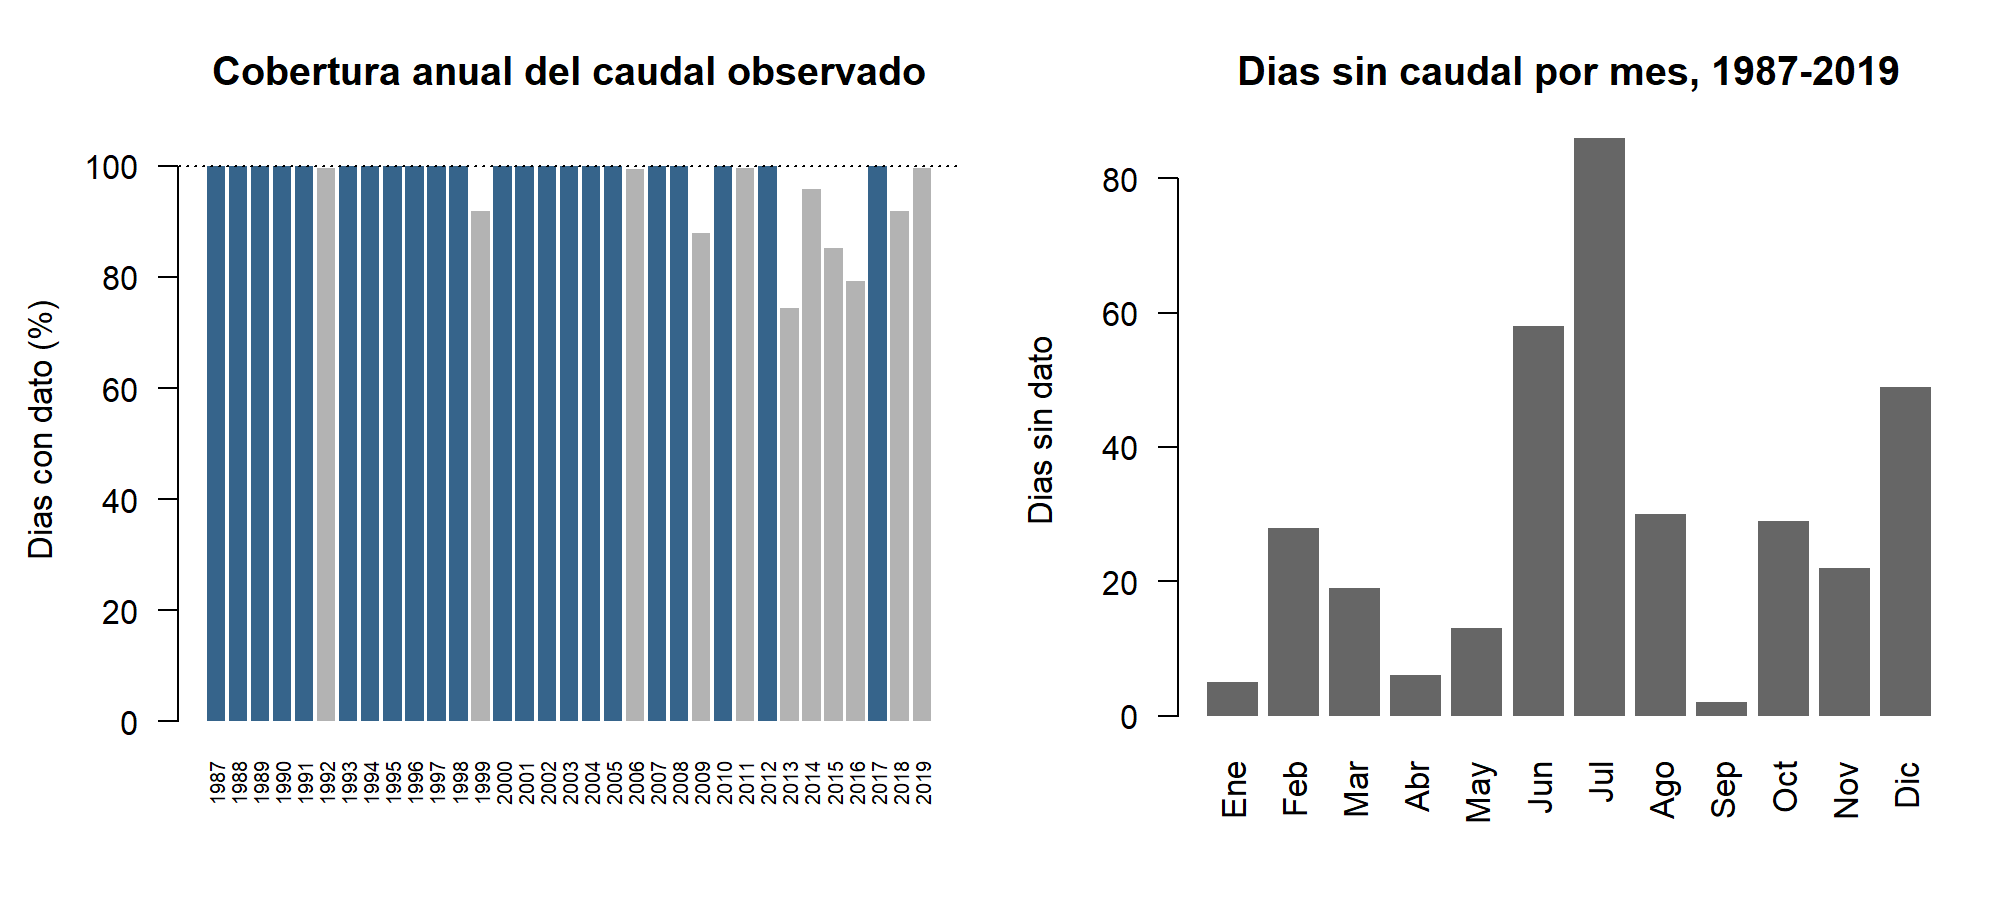
\includegraphics[width=0.95\textwidth]{../03_outputs/figures/05_cobertura_caudal.png}}{%
\fbox{Falta 03\_outputs/figures/05\_cobertura\_caudal.png}}
\caption{Faltantes del caudal DGA observado, antes del relleno. Izquierda:
porcentaje de días con dato en cada año calendario de 1987--2019 (gris: año
incompleto). Derecha: días sin dato por mes del año, sumados en 1987--2019.}
\label{fig:E02faltantes}
\end{figure}

\begin{table}[ht]
\centering
\caption{Controles de calidad y comparación entre fuentes.}
\label{tab:E02controles}
\begin{tabular}{|p{0.42\linewidth}|p{0.16\linewidth}|p{0.27\linewidth}|}
\hline
Control & Período & Resultado \\
\hline
Fechas duplicadas, días faltantes y NA en P, Tmax, Tmin y PET & 1960--2021 & 0 de 22646 días \\
\hline
P negativa, Tmin mayor que Tmax, Tmed fuera de [Tmin, Tmax], PET negativa & 1960--2021 & 0 días \\
\hline
Tmax y Tmin diarias & 1987--2019 & 4.0 a 36.9 °C y $-$6.3 a 16.5 °C \\
\hline
P diaria máxima & 1987--2019 & 85.6 mm\,día$^{-1}$ (2004-04-02) \\
\hline
PET diaria & 1987--2019 & 0.43 a 7.91 mm\,día$^{-1}$ \\
\hline
Q observado diario & 1987--2019 & 0.021 a 157 m$^3$\,s$^{-1}$, sin valores $\le$\,0 \\
\hline
Días sin Q en junio, julio y agosto & 1987--2019 & 174 de 347 \\
\hline
Años calendario con Q observado completo & 1987--2019 & 22 de 33 \\
\hline
Días rellenados por el integrante 2 & 1987--2019 & 314 por regresión con estaciones vecinas (12 bloques), 28 con la mediana de febrero (2009) y 5 por interpolación \\
\hline
Bloques por regresión con error mediano de validación bajo 20 \% & 1987--2019 & 8 de 12; los otros 4, entre 27.7 y 58.9 \% \\
\hline
Días con Q rellenado igual a 0 & 2014-12-17 a 2015-01-04 & 19 \\
\hline
Años calendario con Q completo tras el relleno & 1987--2019 & 33 de 33 \\
\hline
Homogeneidad del Q anual rellenado (integrante 2) & 1987--2019 & sin quiebre: Pettitt $p=$\,0.99, Buishand $p=$\,0.70, SNHT $p=$\,0.27 \\
\hline
P media anual de los 33 años & 1987--2019 & 1601.6 mm\,año$^{-1}$ \\
\hline
P de CR2MET v2.5 frente a la de CAMELS-CL \citep{AlvarezGarreton2018} & 1979-01 a 2020-04 & 1633.9 y 1594.1 mm\,año$^{-1}$ (+2.5 \%); $r=$\,0.992 \\
\hline
PET calculada frente a la de CAMELS-CL & 1979-01 a 2020-04 & 974.3 y 1013.2 mm\,año$^{-1}$ ($-$3.8 \%); $r=$\,0.994 \\
\hline
PET media anual calculada & 1987--2019 & 973.4 mm\,año$^{-1}$ \\
\hline
PET anual en la lámina 12 de \citet{Correa1997} & registros hasta 1991 & sobre 850 mm\,año$^{-1}$ al oeste, cerca de 800 al este \\
\hline
PET anual de las estaciones de \citet{Correa1997} en los bordes de la cuenca & registros hasta 1991 & 827.5 (Cañal Bajo Osorno, oeste) y 701.9 mm\,año$^{-1}$ (Central Pilmaiquén, este) \\
\hline
\end{tabular}
\end{table}

\begin{table}[ht]
\centering
\caption{Prueba de Pettitt \citep{Pettitt1979} sobre las series anuales del
clima, en el período de análisis (1987--2019, 33 años) y en el registro
completo (1960--2021, 62 años). Hipótesis nula: no hay cambio en la mediana
de la serie; la prueba trabaja con los signos de las diferencias entre años,
no con los valores. Nivel de significancia: 5 \%. $p$ por simulación: 999
permutaciones, como en la clase práctica CP05. $p$ aproximado: fórmula
asintótica de \citet{Pettitt1979}, solo como referencia y acotada a 1. Las
medias antes y después del año de quiebre describen el tamaño del cambio.}
\label{tab:E02pettitt}
\begin{tabular}{|p{0.17\linewidth}|p{0.1\linewidth}|p{0.13\linewidth}|p{0.11\linewidth}|p{0.11\linewidth}|p{0.1\linewidth}|p{0.1\linewidth}|}
\hline
Variable & Tramo & Último año\newline antes del\newline quiebre & $p$\newline simulación & $p$\newline aproximado & Media\newline antes & Media\newline después \\
\hline
P (mm\,año$^{-1}$) & 1987--2019 & 1991 & 0.865 & 1 & 1484.1 & 1622.6 \\
\hline
PET (mm\,año$^{-1}$) & 1987--2019 & 2010 & 0.106 & 0.141 & 965.7 & 993.6 \\
\hline
Tmed (°C) & 1987--2019 & 2012 & 0.396 & 0.538 & 11.22 & 11.48 \\
\hline
P (mm\,año$^{-1}$) & 1960--2021 & 1986 & 0.043 & 0.059 & 1761.2 & 1578.7 \\
\hline
PET (mm\,año$^{-1}$) & 1960--2021 & 2010 & 0.026 & 0.047 & 961.1 & 997.4 \\
\hline
Tmed (°C) & 1960--2021 & 1976 & 0.020 & 0.025 & 10.97 & 11.30 \\
\hline
\end{tabular}
\end{table}

\begin{table}[ht]
\centering
\caption{Estacionariedad de las series anuales del clima en 1987--2019 (33
años), con las mismas llamadas de la clase práctica CP05 en el paquete
tseries \citep{tseries}. ADF \citep{SaidDickey1984}: hipótesis nula de raíz
unitaria (serie no estacionaria); incluye intercepto y tendencia, con 4
rezagos. KPSS \citep{Kwiatkowski1992}: hipótesis nula de estacionariedad en
nivel. Nivel de significancia: 5 \%. El paquete acota el $p$ del KPSS a 0.1,
así que 0.1 significa 0.1 o más.}
\label{tab:E02estacionariedad}
\begin{tabular}{|p{0.2\linewidth}|p{0.15\linewidth}|p{0.1\linewidth}|p{0.15\linewidth}|p{0.1\linewidth}|}
\hline
Variable & ADF,\newline estadístico & ADF, $p$ & KPSS,\newline estadístico & KPSS, $p$ \\
\hline
P (mm\,año$^{-1}$) & $-$3.157 & 0.126 & 0.086 & 0.1 \\
\hline
PET (mm\,año$^{-1}$) & $-$2.465 & 0.393 & 0.362 & 0.094 \\
\hline
Tmed (°C) & $-$2.011 & 0.569 & 0.112 & 0.1 \\
\hline
\end{tabular}
\end{table}

\begin{figure}[ht]
\centering
\IfFileExists{../03_outputs/figures/04_PET_mensual_vs_CAMELS.png}{%
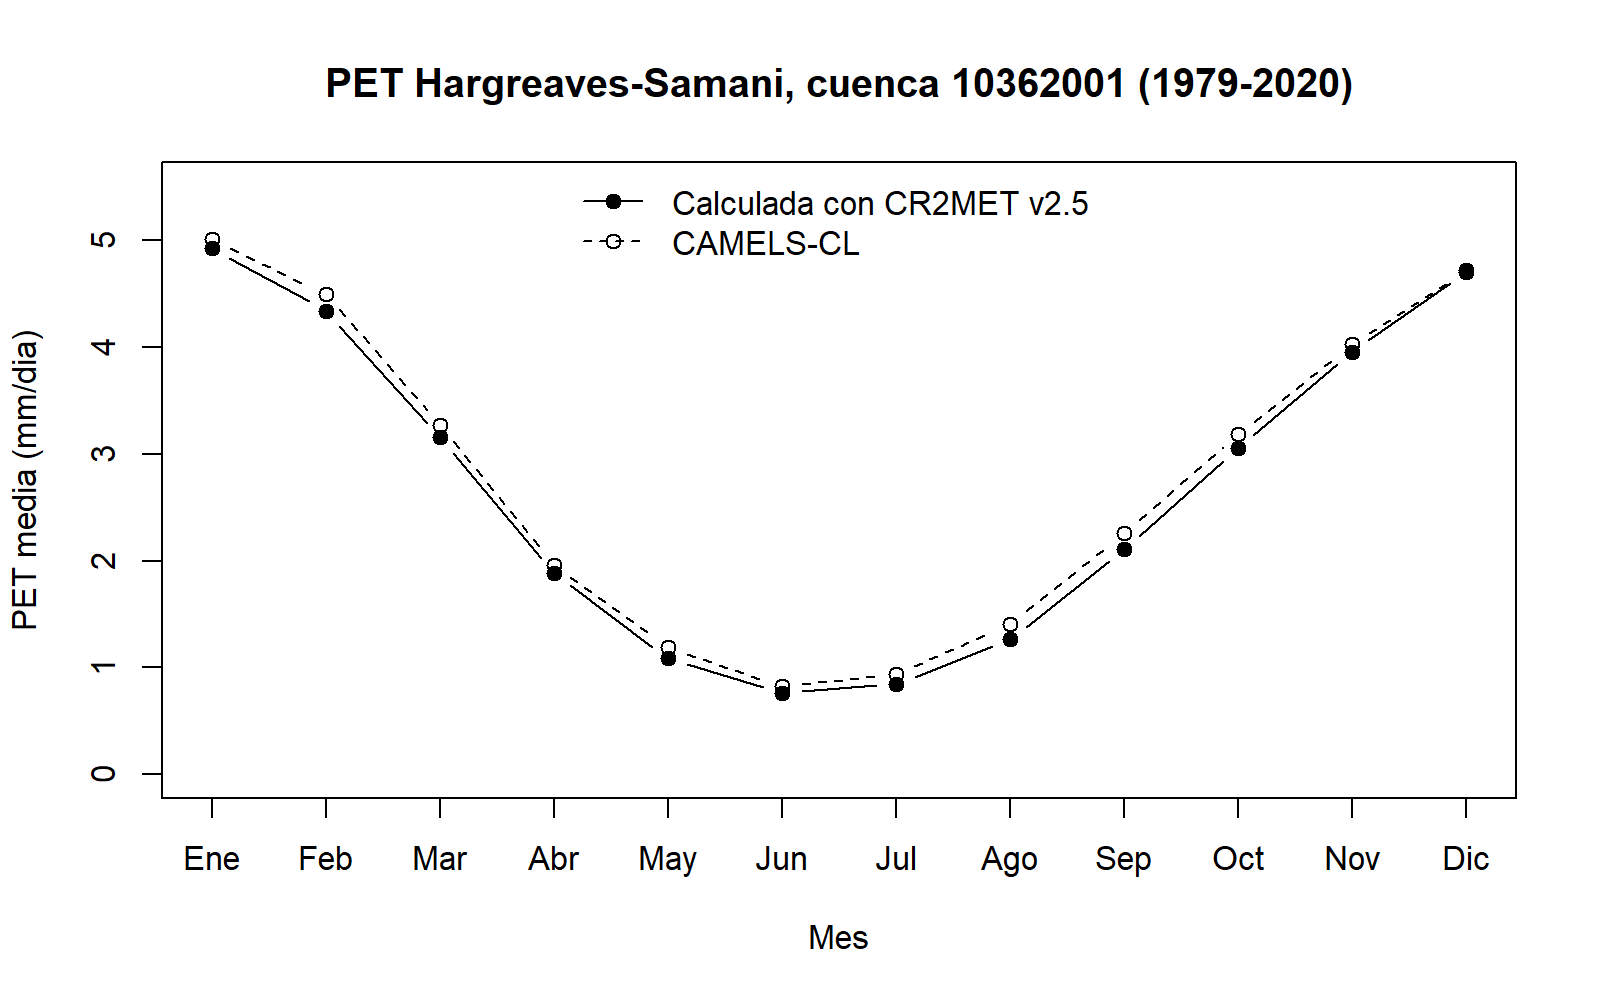
\includegraphics[width=0.8\textwidth]{../03_outputs/figures/04_PET_mensual_vs_CAMELS.png}}{%
\fbox{Falta 03\_outputs/figures/04\_PET\_mensual\_vs\_CAMELS.png}}
\caption{PET media de cada mes del año (mm\,día$^{-1}$), 1979-01 a 2020-04:
calculada con \citet{Hargreaves1985} sobre CR2MET v2.5 y la de CAMELS-CL
\citep{AlvarezGarreton2018}.}
\label{fig:E02pet}
\end{figure}

\campo{3. Fuente y trazabilidad}{Las grillas diarias de CR2MET v2.5 (0.05°,
WGS84) se promedian sobre el polígono de la cuenca delimitado en E01, ponderando cada celda por
la fracción que cae dentro, en \texttt{02\_\allowbreak{}Rscripts/\allowbreak{}04\_\allowbreak{}preparacion\_\allowbreak{}clima.R}.
El mismo script calcula la PET con la ecuación de \citet{Hargreaves1985} y la
radiación extraterrestre de \citet{Allen1998}, a la latitud del centroide del
polígono ($-$40.674°), y hace los controles día a día. La serie queda en
\texttt{01\_\allowbreak{}data/\allowbreak{}processed/\allowbreak{}clima\_\allowbreak{}CR2METv25\_\allowbreak{}10362001\_\allowbreak{}daily\_\allowbreak{}1960-2021.csv}.
El caudal es la serie diaria de la DGA rellenada por el integrante 2 en
\texttt{08b\_\allowbreak{}respaldo\_\allowbreak{}relleno\_\allowbreak{}Q.R} y \texttt{09\_\allowbreak{}consistencia\_\allowbreak{}Q.R}
(\texttt{01\_\allowbreak{}data/\allowbreak{}processed/\allowbreak{}caudal\_\allowbreak{}diario\_\allowbreak{}para\_\allowbreak{}airGR\_\allowbreak{}1987\_\allowbreak{}2019.csv}, que
trae juntas la columna observada, la completada y el método de cada día).
\texttt{02\_\allowbreak{}Rscripts/\allowbreak{}05\_\allowbreak{}regimen\_\allowbreak{}hidroclimatico.R} lo pasa a lámina con el
área del mismo polígono, cuenta los faltantes, aplica las pruebas de Pettitt,
ADF y KPSS (\texttt{05\_\allowbreak{}pettitt\_\allowbreak{}clima\_\allowbreak{}anual.csv} y
\texttt{05\_\allowbreak{}estacionariedad\_\allowbreak{}clima\_\allowbreak{}anual.csv}) y
escribe las cifras de esta ficha en
\texttt{03\_\allowbreak{}outputs/\allowbreak{}tables/\allowbreak{}05\_\allowbreak{}resumen\_\allowbreak{}calidad\_\allowbreak{}E02.csv}. Rutas, polígono y
período se leen de \texttt{06\_\allowbreak{}config/\allowbreak{}parametros.csv}, las fuentes del clima
están en \texttt{04\_\allowbreak{}metadata/\allowbreak{}data\_\allowbreak{}sources.csv} y todo se regenera con
\texttt{run\_\allowbreak{}all.R}.}

\campo{4. Interpretación hidrológica}{El clima no restringe el análisis:
CR2MET v2.5 cubre todos los días de 1960 a 2021 y pasa los controles. En P,
un cero es un día sin lluvia y no un dato faltante: CR2MET no trae NA, y los
controles los cuentan aparte. La variable que define qué años se pueden usar
es el caudal. Sus faltantes no son al azar: la mitad (174 de 347 días) cae
entre junio y agosto, cuando el caudal es mayor (máximo en julio y agosto,
E03). Un caudal anual calculado solo con los días disponibles quedaría bajo,
y descartar los años incompletos dejaría 22 de los 33. El equipo usa la serie
rellenada por el integrante 2: 5 días aislados por interpolación, febrero de
2009 con la mediana de ese mes y 12 bloques (314 días) por regresión con
estaciones vecinas, cada una elegida por validación cruzada. Así los 33 años
quedan completos y entra toda la información del período. El período termina
en 2019 porque 2020 tiene un 69.4 \% de días con caudal; 2021 está completo y
podría sumarse.

Budyko se aplica sobre promedios anuales, y para eso la P y la temperatura
tienen que ser homogéneas y estacionarias en el período que se usa. La prueba
de Pettitt responde si la mediana de una serie cambia en algún año. En
1987--2019 no detecta quiebre en P, PET ni Tmed: el menor $p$ es el de la
PET, 0.106. El KPSS no rechaza la estacionariedad en nivel en ninguna de las
tres ($p\geq$\,0.09; la PET queda cerca del 10 \%) y el ADF no rechaza la
raíz unitaria ($p$ entre 0.126 y 0.569). Las dos pruebas parten de hipótesis
nulas opuestas, aunque no exactamente complementarias: este ADF admite una
tendencia y el KPSS en nivel no. Ninguna muestra que las series dejen de ser
estacionarias, pero el ADF tampoco lo confirma.

En el registro completo sí hay cambios. Tmed sube unos 0.3 °C desde 1977, con
los dos valores $p$ bajo 0.05. La P baja 10 \% desde 1987, con $p=$\,0.043 en
la simulación; la aproximación da 0.059, así que ese quiebre queda en el borde
del 5 \%. El cambio de Tmed es anterior al período de análisis y el de P
coincide con su inicio, de modo que 1987--2019 queda entero después de los
dos. La PET sube 3.8 \% desde 2011 en el registro completo; dentro de
1987--2019 el cambio es de 2.9 \% y no resulta significativo. Las pruebas del
integrante 2 tampoco encuentran quiebre en el caudal anual rellenado.}

\campo{5. Consistencia física}{Los rangos de temperatura y de P diaria son
plausibles para una cuenca templada lluviosa del sur de Chile. Tmed queda
siempre entre Tmin y Tmax y el caudal observado nunca es cero ni negativo. La P de
CR2MET v2.5 difiere en 2.5 \% de la que trae CAMELS-CL (que no declara qué
versión de CR2MET usa), y la PET calculada en $-$3.8 \%, con correlaciones
diarias sobre 0.99. Mes a mes la PET difiere más en invierno, entre $-$7.6 y
$-$10.2 \% de mayo a agosto, cuando sus valores son menores. El orden de
magnitud coincide con el estudio nacional: la PET calculada
(973.4 mm\,año$^{-1}$) supera en 14.5 \% la isolínea de 850 y en 17.6 \% a
Cañal Bajo Osorno.}

\campo{6. Limitaciones e incertidumbre}{No se contrastó CR2MET con una
estación meteorológica dentro de la cuenca, así que la comparación entre
productos mide cuánto difieren, no cuál acierta. Tampoco se puede decir cuál
PET está más cerca de la real. \citet{Correa1997} usaron Penman con la
corrección de FAO-24, que según \citet{Allen1998} puede sobreestimar hasta un
20 \% con baja demanda evaporativa, y la ecuación de \citet{Hargreaves1985}
tiende a sobreestimar con humedad relativa alta \citep{Allen1998}. La PET usa
una sola latitud y se aplica a temperaturas ya promediadas en la cuenca. Con
33 años, un cambio chico como el de la PET dentro del período (2.9 \%) puede
no alcanzar a ser significativo. El ADF se corrió con 4 rezagos, como en la
clase práctica; con 33 años el valor por defecto del paquete sería 3. En 4
de los 12 bloques rellenados por regresión el error mediano de validación va
de 27.7 a 58.9 \%, sobre el 20 \% indicado en clase como límite defendible;
son bloques de verano y comienzos de otoño, con caudales bajos. En el bloque
del 17-12-2014 al 04-01-2015 la regresión dio valores negativos que quedaron
en 0 (19 días). Un caudal nulo no es físico en esta cuenca, cuyo mínimo
observado es 0.021 m$^3$\,s$^{-1}$.}

\campo{7. Conclusión asociada}{Entre 1987 y 2019 el caudal observado cubre el
97.1 \% de los días, pero solo 22 años están completos. Con el relleno del
integrante 2 los 33 años quedan completos y se pueden usar todos en el
balance y en el análisis de Budyko sobre promedios de largo plazo. El clima está completo y difiere menos de 4 \% de CAMELS-CL en
promedio anual. En ese período, P, PET y Tmed no muestran quiebres (Pettitt)
y el KPSS no rechaza su estacionariedad, aunque el ADF no la confirma.}

% Para que los pies digan "Tabla" y no "Cuadro", el preambulo del dossier
% debe decir \PassOptionsToPackage{spanish,es-tabla}{babel}.
% Cifras: 03_outputs/tables/05_resumen_calidad_E02.csv, 04_control_calidad_clima.csv,
% 04_PET_resumen_vs_CAMELS.csv, 04_PET_mensual_vs_CAMELS.csv, 05_pettitt_clima_anual.csv
% y 05_estacionariedad_clima_anual.csv,
% todas generadas por run_all.R.
% Periodo 1987-2019: acordado por el equipo el 19-oct (periodo_inicio y
% periodo_fin en 06_config).
% Fuente del caudal: Mapas DGA, reporte Caudal Diario Historico (fila Q_DGA de data_sources).
% Serie de caudal usada: la rellenada por Alexis (caudal_diario_para_airGR_1987_2019.csv),
% decidido por el equipo el 19-oct.
% Poligono: el de Alexis (cuenca_rio_damas.gpkg), desde el 19-oct.

\section{E02. Calidad y cobertura de la información}
\label{ev:E02}

\campo{1. Pregunta o afirmación que se evalúa}{¿Son suficientes y
consistentes la precipitación, las temperaturas, la PET y el caudal para
compararlos año a año en el período de análisis 1987--2019?}

\campo{2. Evidencia principal}{La Tabla~\ref{tab:E02cobertura} resume la
fuente, el registro y la cobertura de cada variable, y la
Figura~\ref{fig:E02faltantes} muestra dónde están los días sin caudal. La
Tabla~\ref{tab:E02controles} reúne los controles y las comparaciones con
otras fuentes. Las Tablas~\ref{tab:E02pettitt} y~\ref{tab:E02estacionariedad}
muestran las pruebas de homogeneidad y estacionariedad de las series anuales
del clima. La Figura~\ref{fig:E02pet} compara el ciclo
anual de la PET calculada con el de CAMELS-CL.}

\begin{table}[ht]
\centering
\caption{Fuente, registro y cobertura por variable. Cobertura: porcentaje de
días con dato dentro de 1987--2019.}
\label{tab:E02cobertura}
\begin{tabular}{|p{0.17\linewidth}|p{0.32\linewidth}|p{0.17\linewidth}|p{0.16\linewidth}|}
\hline
Variable (unidad) & Fuente & Registro & Cobertura 1987--2019, en \% \\
\hline
P (mm\,día$^{-1}$) & CR2MET v2.5 \citep{Boisier2023} & 1960-01-01 a 2021-12-31 & 100 \\
\hline
Tmax, Tmin (°C) & CR2MET v2.5 \citep{Boisier2023} & 1960-01-01 a 2021-12-31 & 100 \\
\hline
Tmed (°C) & (Tmax + Tmin)/2 & 1960-01-01 a 2021-12-31 & 100 \\
\hline
PET (mm\,día$^{-1}$) & \citet{Hargreaves1985} con Tmax y Tmin de CR2MET v2.5 & 1960-01-01 a 2021-12-31 & 100 \\
\hline
Q (m$^3$\,s$^{-1}$) & DGA, estación Río Damas en Tacamo \citep{DGA_mapas}, rellenada por el integrante 2 & 1986-02-01 a 2026-06-15 & 97.12 observado (347 días sin dato); 100 con el relleno \\
\hline
\end{tabular}
\end{table}

\begin{figure}[ht]
\centering
\IfFileExists{../03_outputs/figures/05_cobertura_caudal.png}{%
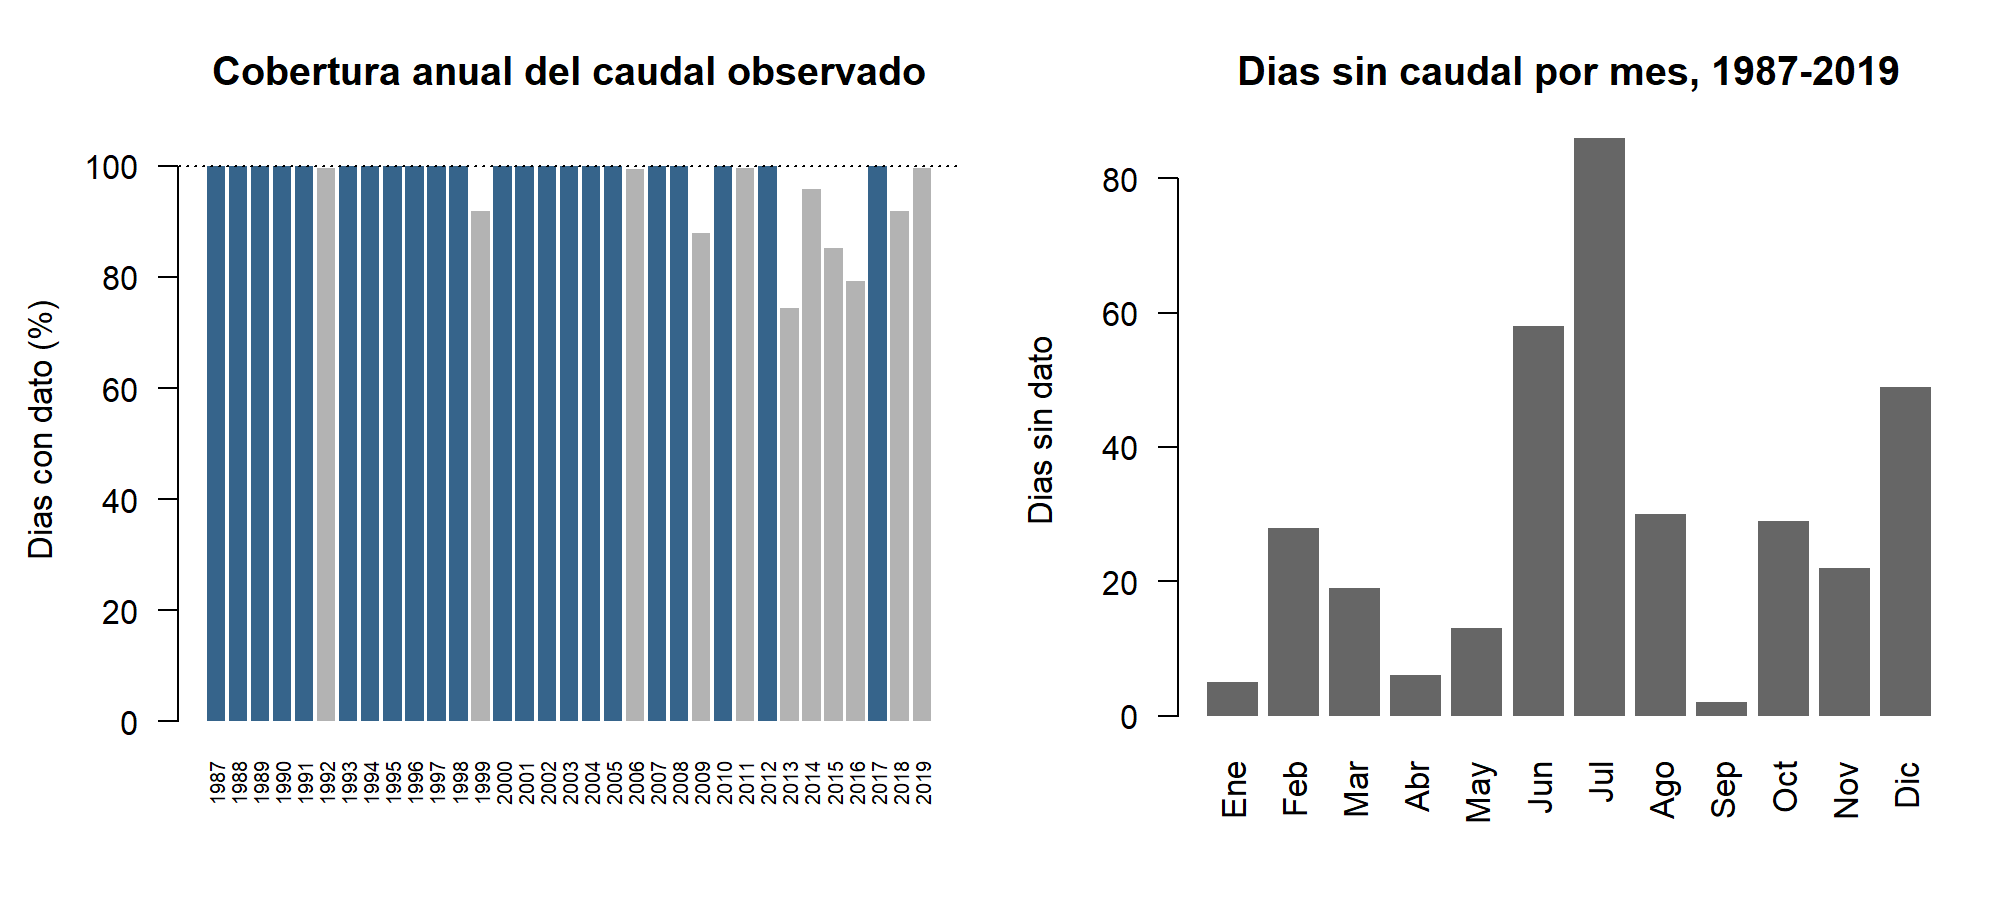
\includegraphics[width=0.95\textwidth]{../03_outputs/figures/05_cobertura_caudal.png}}{%
\fbox{Falta 03\_outputs/figures/05\_cobertura\_caudal.png}}
\caption{Faltantes del caudal DGA observado, antes del relleno. Izquierda:
porcentaje de días con dato en cada año calendario de 1987--2019 (gris: año
incompleto). Derecha: días sin dato por mes del año, sumados en 1987--2019.}
\label{fig:E02faltantes}
\end{figure}

\begin{table}[ht]
\centering
\caption{Controles de calidad y comparación entre fuentes.}
\label{tab:E02controles}
\begin{tabular}{|p{0.42\linewidth}|p{0.16\linewidth}|p{0.27\linewidth}|}
\hline
Control & Período & Resultado \\
\hline
Fechas duplicadas, días faltantes y NA en P, Tmax, Tmin y PET & 1960--2021 & 0 de 22646 días \\
\hline
P negativa, Tmin mayor que Tmax, Tmed fuera de [Tmin, Tmax], PET negativa & 1960--2021 & 0 días \\
\hline
Tmax y Tmin diarias & 1987--2019 & 4.0 a 36.9 °C y $-$6.3 a 16.5 °C \\
\hline
P diaria máxima & 1987--2019 & 85.6 mm\,día$^{-1}$ (2004-04-02) \\
\hline
PET diaria & 1987--2019 & 0.43 a 7.91 mm\,día$^{-1}$ \\
\hline
Q observado diario & 1987--2019 & 0.021 a 157 m$^3$\,s$^{-1}$, sin valores $\le$\,0 \\
\hline
Días sin Q en junio, julio y agosto & 1987--2019 & 174 de 347 \\
\hline
Años calendario con Q observado completo & 1987--2019 & 22 de 33 \\
\hline
Días rellenados por el integrante 2 & 1987--2019 & 314 por regresión con estaciones vecinas (12 bloques), 28 con la mediana de febrero (2009) y 5 por interpolación \\
\hline
Bloques por regresión con error mediano de validación bajo 20 \% & 1987--2019 & 8 de 12; los otros 4, entre 27.7 y 58.9 \% \\
\hline
Días con Q rellenado igual a 0 & 2014-12-17 a 2015-01-04 & 19 \\
\hline
Años calendario con Q completo tras el relleno & 1987--2019 & 33 de 33 \\
\hline
Homogeneidad del Q anual rellenado (integrante 2) & 1987--2019 & sin quiebre: Pettitt $p=$\,0.99, Buishand $p=$\,0.70, SNHT $p=$\,0.27 \\
\hline
P media anual de los 33 años & 1987--2019 & 1601.6 mm\,año$^{-1}$ \\
\hline
P de CR2MET v2.5 frente a la de CAMELS-CL \citep{AlvarezGarreton2018} & 1979-01 a 2020-04 & 1633.9 y 1594.1 mm\,año$^{-1}$ (+2.5 \%); $r=$\,0.992 \\
\hline
PET calculada frente a la de CAMELS-CL & 1979-01 a 2020-04 & 974.3 y 1013.2 mm\,año$^{-1}$ ($-$3.8 \%); $r=$\,0.994 \\
\hline
PET media anual calculada & 1987--2019 & 973.4 mm\,año$^{-1}$ \\
\hline
PET anual en la lámina 12 de \citet{Correa1997} & registros hasta 1991 & sobre 850 mm\,año$^{-1}$ al oeste, cerca de 800 al este \\
\hline
PET anual de las estaciones de \citet{Correa1997} en los bordes de la cuenca & registros hasta 1991 & 827.5 (Cañal Bajo Osorno, oeste) y 701.9 mm\,año$^{-1}$ (Central Pilmaiquén, este) \\
\hline
\end{tabular}
\end{table}

\begin{table}[ht]
\centering
\caption{Prueba de Pettitt \citep{Pettitt1979} sobre las series anuales del
clima, en el período de análisis (1987--2019, 33 años) y en el registro
completo (1960--2021, 62 años). Hipótesis nula: no hay cambio en la mediana
de la serie; la prueba trabaja con los signos de las diferencias entre años,
no con los valores. Nivel de significancia: 5 \%. $p$ por simulación: 999
permutaciones, como en la clase práctica CP05. $p$ aproximado: fórmula
asintótica de \citet{Pettitt1979}, solo como referencia y acotada a 1. Las
medias antes y después del año de quiebre describen el tamaño del cambio.}
\label{tab:E02pettitt}
\begin{tabular}{|p{0.17\linewidth}|p{0.1\linewidth}|p{0.13\linewidth}|p{0.11\linewidth}|p{0.11\linewidth}|p{0.1\linewidth}|p{0.1\linewidth}|}
\hline
Variable & Tramo & Último año\newline antes del\newline quiebre & $p$\newline simulación & $p$\newline aproximado & Media\newline antes & Media\newline después \\
\hline
P (mm\,año$^{-1}$) & 1987--2019 & 1991 & 0.865 & 1 & 1484.1 & 1622.6 \\
\hline
PET (mm\,año$^{-1}$) & 1987--2019 & 2010 & 0.106 & 0.141 & 965.7 & 993.6 \\
\hline
Tmed (°C) & 1987--2019 & 2012 & 0.396 & 0.538 & 11.22 & 11.48 \\
\hline
P (mm\,año$^{-1}$) & 1960--2021 & 1986 & 0.043 & 0.059 & 1761.2 & 1578.7 \\
\hline
PET (mm\,año$^{-1}$) & 1960--2021 & 2010 & 0.026 & 0.047 & 961.1 & 997.4 \\
\hline
Tmed (°C) & 1960--2021 & 1976 & 0.020 & 0.025 & 10.97 & 11.30 \\
\hline
\end{tabular}
\end{table}

\begin{table}[ht]
\centering
\caption{Estacionariedad de las series anuales del clima en 1987--2019 (33
años), con las mismas llamadas de la clase práctica CP05 en el paquete
tseries \citep{tseries}. ADF \citep{SaidDickey1984}: hipótesis nula de raíz
unitaria (serie no estacionaria); incluye intercepto y tendencia, con 4
rezagos. KPSS \citep{Kwiatkowski1992}: hipótesis nula de estacionariedad en
nivel. Nivel de significancia: 5 \%. El paquete acota el $p$ del KPSS a 0.1,
así que 0.1 significa 0.1 o más.}
\label{tab:E02estacionariedad}
\begin{tabular}{|p{0.2\linewidth}|p{0.15\linewidth}|p{0.1\linewidth}|p{0.15\linewidth}|p{0.1\linewidth}|}
\hline
Variable & ADF,\newline estadístico & ADF, $p$ & KPSS,\newline estadístico & KPSS, $p$ \\
\hline
P (mm\,año$^{-1}$) & $-$3.157 & 0.126 & 0.086 & 0.1 \\
\hline
PET (mm\,año$^{-1}$) & $-$2.465 & 0.393 & 0.362 & 0.094 \\
\hline
Tmed (°C) & $-$2.011 & 0.569 & 0.112 & 0.1 \\
\hline
\end{tabular}
\end{table}

\begin{figure}[ht]
\centering
\IfFileExists{../03_outputs/figures/04_PET_mensual_vs_CAMELS.png}{%
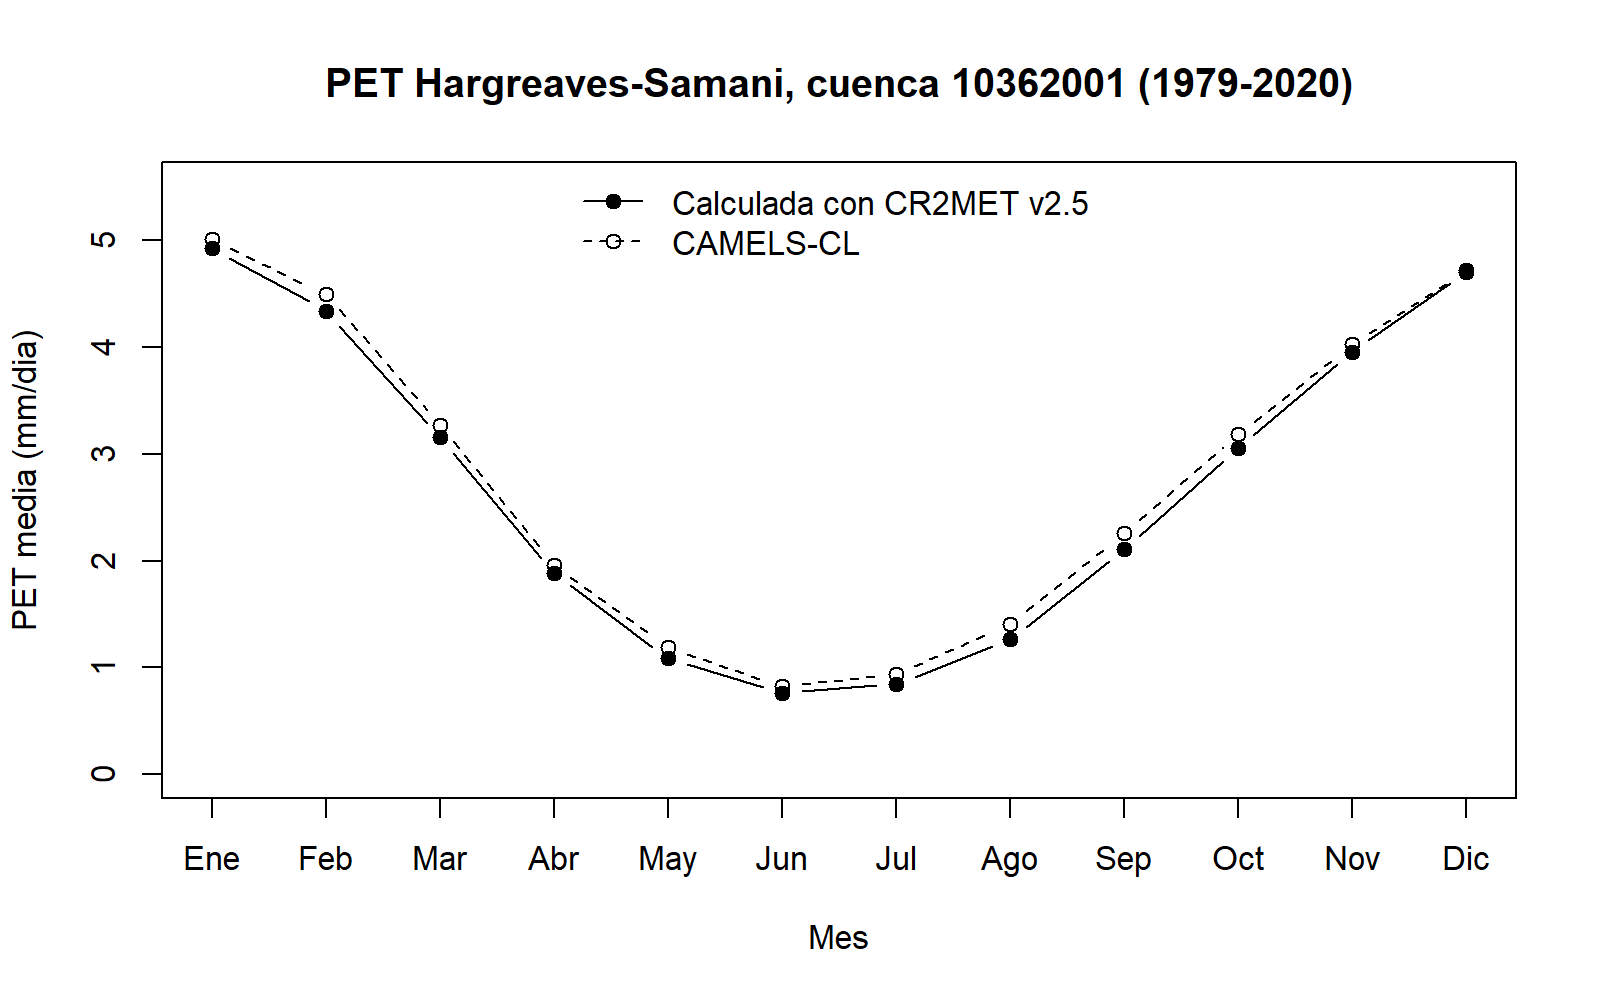
\includegraphics[width=0.8\textwidth]{../03_outputs/figures/04_PET_mensual_vs_CAMELS.png}}{%
\fbox{Falta 03\_outputs/figures/04\_PET\_mensual\_vs\_CAMELS.png}}
\caption{PET media de cada mes del año (mm\,día$^{-1}$), 1979-01 a 2020-04:
calculada con \citet{Hargreaves1985} sobre CR2MET v2.5 y la de CAMELS-CL
\citep{AlvarezGarreton2018}.}
\label{fig:E02pet}
\end{figure}

\campo{3. Fuente y trazabilidad}{Las grillas diarias de CR2MET v2.5 (0.05°,
WGS84) se promedian sobre el polígono de la cuenca delimitado en E01, ponderando cada celda por
la fracción que cae dentro, en \texttt{02\_\allowbreak{}Rscripts/\allowbreak{}04\_\allowbreak{}preparacion\_\allowbreak{}clima.R}.
El mismo script calcula la PET con la ecuación de \citet{Hargreaves1985} y la
radiación extraterrestre de \citet{Allen1998}, a la latitud del centroide del
polígono ($-$40.674°), y hace los controles día a día. La serie queda en
\texttt{01\_\allowbreak{}data/\allowbreak{}processed/\allowbreak{}clima\_\allowbreak{}CR2METv25\_\allowbreak{}10362001\_\allowbreak{}daily\_\allowbreak{}1960-2021.csv}.
El caudal es la serie diaria de la DGA rellenada por el integrante 2 en
\texttt{08b\_\allowbreak{}respaldo\_\allowbreak{}relleno\_\allowbreak{}Q.R} y \texttt{09\_\allowbreak{}consistencia\_\allowbreak{}Q.R}
(\texttt{01\_\allowbreak{}data/\allowbreak{}processed/\allowbreak{}caudal\_\allowbreak{}diario\_\allowbreak{}para\_\allowbreak{}airGR\_\allowbreak{}1987\_\allowbreak{}2019.csv}, que
trae juntas la columna observada, la completada y el método de cada día).
\texttt{02\_\allowbreak{}Rscripts/\allowbreak{}05\_\allowbreak{}regimen\_\allowbreak{}hidroclimatico.R} lo pasa a lámina con el
área del mismo polígono, cuenta los faltantes, aplica las pruebas de Pettitt,
ADF y KPSS (\texttt{05\_\allowbreak{}pettitt\_\allowbreak{}clima\_\allowbreak{}anual.csv} y
\texttt{05\_\allowbreak{}estacionariedad\_\allowbreak{}clima\_\allowbreak{}anual.csv}) y
escribe las cifras de esta ficha en
\texttt{03\_\allowbreak{}outputs/\allowbreak{}tables/\allowbreak{}05\_\allowbreak{}resumen\_\allowbreak{}calidad\_\allowbreak{}E02.csv}. Rutas, polígono y
período se leen de \texttt{06\_\allowbreak{}config/\allowbreak{}parametros.csv}, las fuentes del clima
están en \texttt{04\_\allowbreak{}metadata/\allowbreak{}data\_\allowbreak{}sources.csv} y todo se regenera con
\texttt{run\_\allowbreak{}all.R}.}

\campo{4. Interpretación hidrológica}{El clima no restringe el análisis:
CR2MET v2.5 cubre todos los días de 1960 a 2021 y pasa los controles. En P,
un cero es un día sin lluvia y no un dato faltante: CR2MET no trae NA, y los
controles los cuentan aparte. La variable que define qué años se pueden usar
es el caudal. Sus faltantes no son al azar: la mitad (174 de 347 días) cae
entre junio y agosto, cuando el caudal es mayor (máximo en julio y agosto,
E03). Un caudal anual calculado solo con los días disponibles quedaría bajo,
y descartar los años incompletos dejaría 22 de los 33. El equipo usa la serie
rellenada por el integrante 2: 5 días aislados por interpolación, febrero de
2009 con la mediana de ese mes y 12 bloques (314 días) por regresión con
estaciones vecinas, cada una elegida por validación cruzada. Así los 33 años
quedan completos y entra toda la información del período. El período termina
en 2019 porque 2020 tiene un 69.4 \% de días con caudal; 2021 está completo y
podría sumarse.

Budyko se aplica sobre promedios anuales, y para eso la P y la temperatura
tienen que ser homogéneas y estacionarias en el período que se usa. La prueba
de Pettitt responde si la mediana de una serie cambia en algún año. En
1987--2019 no detecta quiebre en P, PET ni Tmed: el menor $p$ es el de la
PET, 0.106. El KPSS no rechaza la estacionariedad en nivel en ninguna de las
tres ($p\geq$\,0.09; la PET queda cerca del 10 \%) y el ADF no rechaza la
raíz unitaria ($p$ entre 0.126 y 0.569). Las dos pruebas parten de hipótesis
nulas opuestas, aunque no exactamente complementarias: este ADF admite una
tendencia y el KPSS en nivel no. Ninguna muestra que las series dejen de ser
estacionarias, pero el ADF tampoco lo confirma.

En el registro completo sí hay cambios. Tmed sube unos 0.3 °C desde 1977, con
los dos valores $p$ bajo 0.05. La P baja 10 \% desde 1987, con $p=$\,0.043 en
la simulación; la aproximación da 0.059, así que ese quiebre queda en el borde
del 5 \%. El cambio de Tmed es anterior al período de análisis y el de P
coincide con su inicio, de modo que 1987--2019 queda entero después de los
dos. La PET sube 3.8 \% desde 2011 en el registro completo; dentro de
1987--2019 el cambio es de 2.9 \% y no resulta significativo. Las pruebas del
integrante 2 tampoco encuentran quiebre en el caudal anual rellenado.}

\campo{5. Consistencia física}{Los rangos de temperatura y de P diaria son
plausibles para una cuenca templada lluviosa del sur de Chile. Tmed queda
siempre entre Tmin y Tmax y el caudal observado nunca es cero ni negativo. La P de
CR2MET v2.5 difiere en 2.5 \% de la que trae CAMELS-CL (que no declara qué
versión de CR2MET usa), y la PET calculada en $-$3.8 \%, con correlaciones
diarias sobre 0.99. Mes a mes la PET difiere más en invierno, entre $-$7.6 y
$-$10.2 \% de mayo a agosto, cuando sus valores son menores. El orden de
magnitud coincide con el estudio nacional: la PET calculada
(973.4 mm\,año$^{-1}$) supera en 14.5 \% la isolínea de 850 y en 17.6 \% a
Cañal Bajo Osorno.}

\campo{6. Limitaciones e incertidumbre}{No se contrastó CR2MET con una
estación meteorológica dentro de la cuenca, así que la comparación entre
productos mide cuánto difieren, no cuál acierta. Tampoco se puede decir cuál
PET está más cerca de la real. \citet{Correa1997} usaron Penman con la
corrección de FAO-24, que según \citet{Allen1998} puede sobreestimar hasta un
20 \% con baja demanda evaporativa, y la ecuación de \citet{Hargreaves1985}
tiende a sobreestimar con humedad relativa alta \citep{Allen1998}. La PET usa
una sola latitud y se aplica a temperaturas ya promediadas en la cuenca. Con
33 años, un cambio chico como el de la PET dentro del período (2.9 \%) puede
no alcanzar a ser significativo. El ADF se corrió con 4 rezagos, como en la
clase práctica; con 33 años el valor por defecto del paquete sería 3. En 4
de los 12 bloques rellenados por regresión el error mediano de validación va
de 27.7 a 58.9 \%, sobre el 20 \% indicado en clase como límite defendible;
son bloques de verano y comienzos de otoño, con caudales bajos. En el bloque
del 17-12-2014 al 04-01-2015 la regresión dio valores negativos que quedaron
en 0 (19 días). Un caudal nulo no es físico en esta cuenca, cuyo mínimo
observado es 0.021 m$^3$\,s$^{-1}$.}

\campo{7. Conclusión asociada}{Entre 1987 y 2019 el caudal observado cubre el
97.1 \% de los días, pero solo 22 años están completos. Con el relleno del
integrante 2 los 33 años quedan completos y se pueden usar todos en el
balance y en el análisis de Budyko sobre promedios de largo plazo. El clima está completo y difiere menos de 4 \% de CAMELS-CL en
promedio anual. En ese período, P, PET y Tmed no muestran quiebres (Pettitt)
y el KPSS no rechaza su estacionariedad, aunque el ADF no la confirma.}

% Para que los pies digan "Tabla" y no "Cuadro", el preambulo del dossier
% debe decir \PassOptionsToPackage{spanish,es-tabla}{babel}.
% Cifras: 03_outputs/tables/05_resumen_calidad_E02.csv, 04_control_calidad_clima.csv,
% 04_PET_resumen_vs_CAMELS.csv, 04_PET_mensual_vs_CAMELS.csv, 05_pettitt_clima_anual.csv
% y 05_estacionariedad_clima_anual.csv,
% todas generadas por run_all.R.
% Periodo 1987-2019: acordado por el equipo el 19-oct (periodo_inicio y
% periodo_fin en 06_config).
% Fuente del caudal: Mapas DGA, reporte Caudal Diario Historico (fila Q_DGA de data_sources).
% Serie de caudal usada: la rellenada por Alexis (caudal_diario_para_airGR_1987_2019.csv),
% decidido por el equipo el 19-oct.
% Poligono: el de Alexis (cuenca_rio_damas.gpkg), desde el 19-oct.

\section{E02. Calidad y cobertura de la información}
\label{ev:E02}

\campo{1. Pregunta o afirmación que se evalúa}{¿Son suficientes y
consistentes la precipitación, las temperaturas, la PET y el caudal para
compararlos año a año en el período de análisis 1987--2019?}

\campo{2. Evidencia principal}{La Tabla~\ref{tab:E02cobertura} resume la
fuente, el registro y la cobertura de cada variable, y la
Figura~\ref{fig:E02faltantes} muestra dónde están los días sin caudal. La
Tabla~\ref{tab:E02controles} reúne los controles y las comparaciones con
otras fuentes. Las Tablas~\ref{tab:E02pettitt} y~\ref{tab:E02estacionariedad}
muestran las pruebas de homogeneidad y estacionariedad de las series anuales
del clima. La Figura~\ref{fig:E02pet} compara el ciclo
anual de la PET calculada con el de CAMELS-CL.}

\begin{table}[ht]
\centering
\caption{Fuente, registro y cobertura por variable. Cobertura: porcentaje de
días con dato dentro de 1987--2019.}
\label{tab:E02cobertura}
\begin{tabular}{|p{0.17\linewidth}|p{0.32\linewidth}|p{0.17\linewidth}|p{0.16\linewidth}|}
\hline
Variable (unidad) & Fuente & Registro & Cobertura 1987--2019, en \% \\
\hline
P (mm\,día$^{-1}$) & CR2MET v2.5 \citep{Boisier2023} & 1960-01-01 a 2021-12-31 & 100 \\
\hline
Tmax, Tmin (°C) & CR2MET v2.5 \citep{Boisier2023} & 1960-01-01 a 2021-12-31 & 100 \\
\hline
Tmed (°C) & (Tmax + Tmin)/2 & 1960-01-01 a 2021-12-31 & 100 \\
\hline
PET (mm\,día$^{-1}$) & \citet{Hargreaves1985} con Tmax y Tmin de CR2MET v2.5 & 1960-01-01 a 2021-12-31 & 100 \\
\hline
Q (m$^3$\,s$^{-1}$) & DGA, estación Río Damas en Tacamo \citep{DGA_mapas}, rellenada por el integrante 2 & 1986-02-01 a 2026-06-15 & 97.12 observado (347 días sin dato); 100 con el relleno \\
\hline
\end{tabular}
\end{table}

\begin{figure}[ht]
\centering
\IfFileExists{../03_outputs/figures/05_cobertura_caudal.png}{%
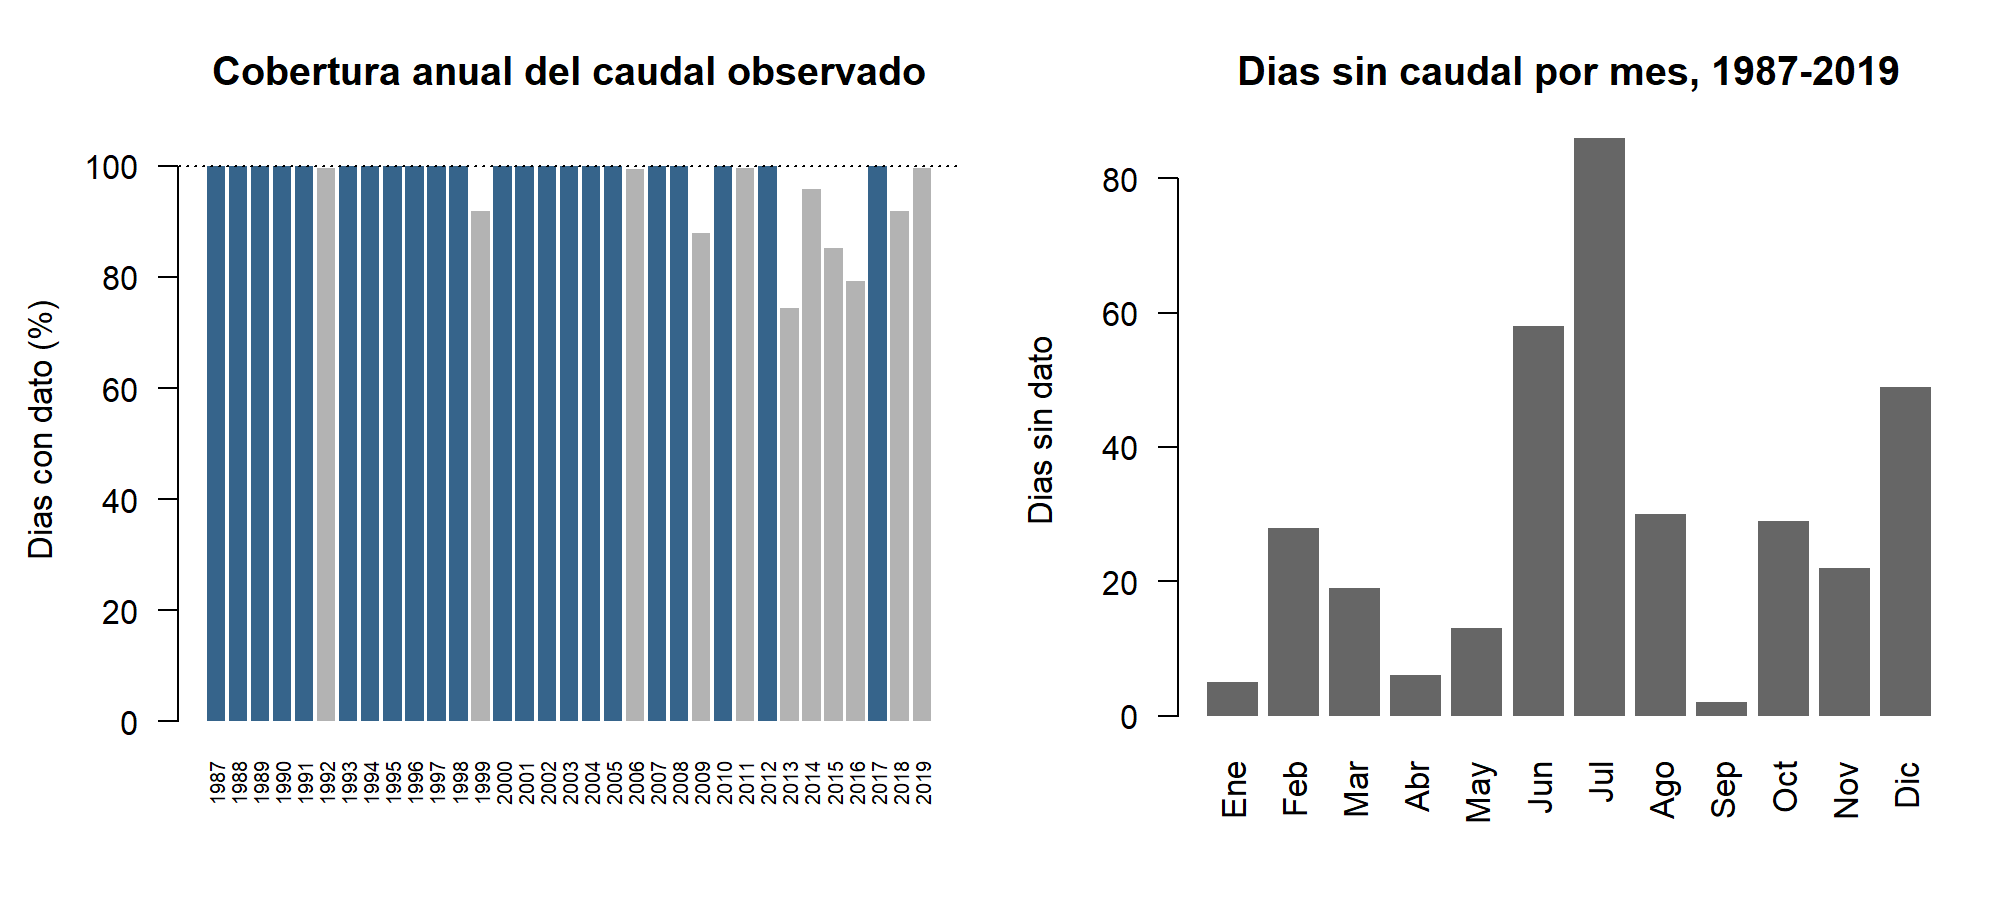
\includegraphics[width=0.95\textwidth]{../03_outputs/figures/05_cobertura_caudal.png}}{%
\fbox{Falta 03\_outputs/figures/05\_cobertura\_caudal.png}}
\caption{Faltantes del caudal DGA observado, antes del relleno. Izquierda:
porcentaje de días con dato en cada año calendario de 1987--2019 (gris: año
incompleto). Derecha: días sin dato por mes del año, sumados en 1987--2019.}
\label{fig:E02faltantes}
\end{figure}

\begin{table}[ht]
\centering
\caption{Controles de calidad y comparación entre fuentes.}
\label{tab:E02controles}
\begin{tabular}{|p{0.42\linewidth}|p{0.16\linewidth}|p{0.27\linewidth}|}
\hline
Control & Período & Resultado \\
\hline
Fechas duplicadas, días faltantes y NA en P, Tmax, Tmin y PET & 1960--2021 & 0 de 22646 días \\
\hline
P negativa, Tmin mayor que Tmax, Tmed fuera de [Tmin, Tmax], PET negativa & 1960--2021 & 0 días \\
\hline
Tmax y Tmin diarias & 1987--2019 & 4.0 a 36.9 °C y $-$6.3 a 16.5 °C \\
\hline
P diaria máxima & 1987--2019 & 85.6 mm\,día$^{-1}$ (2004-04-02) \\
\hline
PET diaria & 1987--2019 & 0.43 a 7.91 mm\,día$^{-1}$ \\
\hline
Q observado diario & 1987--2019 & 0.021 a 157 m$^3$\,s$^{-1}$, sin valores $\le$\,0 \\
\hline
Días sin Q en junio, julio y agosto & 1987--2019 & 174 de 347 \\
\hline
Años calendario con Q observado completo & 1987--2019 & 22 de 33 \\
\hline
Días rellenados por el integrante 2 & 1987--2019 & 314 por regresión con estaciones vecinas (12 bloques), 28 con la mediana de febrero (2009) y 5 por interpolación \\
\hline
Bloques por regresión con error mediano de validación bajo 20 \% & 1987--2019 & 8 de 12; los otros 4, entre 27.7 y 58.9 \% \\
\hline
Días con Q rellenado igual a 0 & 2014-12-17 a 2015-01-04 & 19 \\
\hline
Años calendario con Q completo tras el relleno & 1987--2019 & 33 de 33 \\
\hline
Homogeneidad del Q anual rellenado (integrante 2) & 1987--2019 & sin quiebre: Pettitt $p=$\,0.99, Buishand $p=$\,0.70, SNHT $p=$\,0.27 \\
\hline
P media anual de los 33 años & 1987--2019 & 1601.6 mm\,año$^{-1}$ \\
\hline
P de CR2MET v2.5 frente a la de CAMELS-CL \citep{AlvarezGarreton2018} & 1979-01 a 2020-04 & 1633.9 y 1594.1 mm\,año$^{-1}$ (+2.5 \%); $r=$\,0.992 \\
\hline
PET calculada frente a la de CAMELS-CL & 1979-01 a 2020-04 & 974.3 y 1013.2 mm\,año$^{-1}$ ($-$3.8 \%); $r=$\,0.994 \\
\hline
PET media anual calculada & 1987--2019 & 973.4 mm\,año$^{-1}$ \\
\hline
PET anual en la lámina 12 de \citet{Correa1997} & registros hasta 1991 & sobre 850 mm\,año$^{-1}$ al oeste, cerca de 800 al este \\
\hline
PET anual de las estaciones de \citet{Correa1997} en los bordes de la cuenca & registros hasta 1991 & 827.5 (Cañal Bajo Osorno, oeste) y 701.9 mm\,año$^{-1}$ (Central Pilmaiquén, este) \\
\hline
\end{tabular}
\end{table}

\begin{table}[ht]
\centering
\caption{Prueba de Pettitt \citep{Pettitt1979} sobre las series anuales del
clima, en el período de análisis (1987--2019, 33 años) y en el registro
completo (1960--2021, 62 años). Hipótesis nula: no hay cambio en la mediana
de la serie; la prueba trabaja con los signos de las diferencias entre años,
no con los valores. Nivel de significancia: 5 \%. $p$ por simulación: 999
permutaciones, como en la clase práctica CP05. $p$ aproximado: fórmula
asintótica de \citet{Pettitt1979}, solo como referencia y acotada a 1. Las
medias antes y después del año de quiebre describen el tamaño del cambio.}
\label{tab:E02pettitt}
\begin{tabular}{|p{0.17\linewidth}|p{0.1\linewidth}|p{0.13\linewidth}|p{0.11\linewidth}|p{0.11\linewidth}|p{0.1\linewidth}|p{0.1\linewidth}|}
\hline
Variable & Tramo & Último año\newline antes del\newline quiebre & $p$\newline simulación & $p$\newline aproximado & Media\newline antes & Media\newline después \\
\hline
P (mm\,año$^{-1}$) & 1987--2019 & 1991 & 0.865 & 1 & 1484.1 & 1622.6 \\
\hline
PET (mm\,año$^{-1}$) & 1987--2019 & 2010 & 0.106 & 0.141 & 965.7 & 993.6 \\
\hline
Tmed (°C) & 1987--2019 & 2012 & 0.396 & 0.538 & 11.22 & 11.48 \\
\hline
P (mm\,año$^{-1}$) & 1960--2021 & 1986 & 0.043 & 0.059 & 1761.2 & 1578.7 \\
\hline
PET (mm\,año$^{-1}$) & 1960--2021 & 2010 & 0.026 & 0.047 & 961.1 & 997.4 \\
\hline
Tmed (°C) & 1960--2021 & 1976 & 0.020 & 0.025 & 10.97 & 11.30 \\
\hline
\end{tabular}
\end{table}

\begin{table}[ht]
\centering
\caption{Estacionariedad de las series anuales del clima en 1987--2019 (33
años), con las mismas llamadas de la clase práctica CP05 en el paquete
tseries \citep{tseries}. ADF \citep{SaidDickey1984}: hipótesis nula de raíz
unitaria (serie no estacionaria); incluye intercepto y tendencia, con 4
rezagos. KPSS \citep{Kwiatkowski1992}: hipótesis nula de estacionariedad en
nivel. Nivel de significancia: 5 \%. El paquete acota el $p$ del KPSS a 0.1,
así que 0.1 significa 0.1 o más.}
\label{tab:E02estacionariedad}
\begin{tabular}{|p{0.2\linewidth}|p{0.15\linewidth}|p{0.1\linewidth}|p{0.15\linewidth}|p{0.1\linewidth}|}
\hline
Variable & ADF,\newline estadístico & ADF, $p$ & KPSS,\newline estadístico & KPSS, $p$ \\
\hline
P (mm\,año$^{-1}$) & $-$3.157 & 0.126 & 0.086 & 0.1 \\
\hline
PET (mm\,año$^{-1}$) & $-$2.465 & 0.393 & 0.362 & 0.094 \\
\hline
Tmed (°C) & $-$2.011 & 0.569 & 0.112 & 0.1 \\
\hline
\end{tabular}
\end{table}

\begin{figure}[ht]
\centering
\IfFileExists{../03_outputs/figures/04_PET_mensual_vs_CAMELS.png}{%
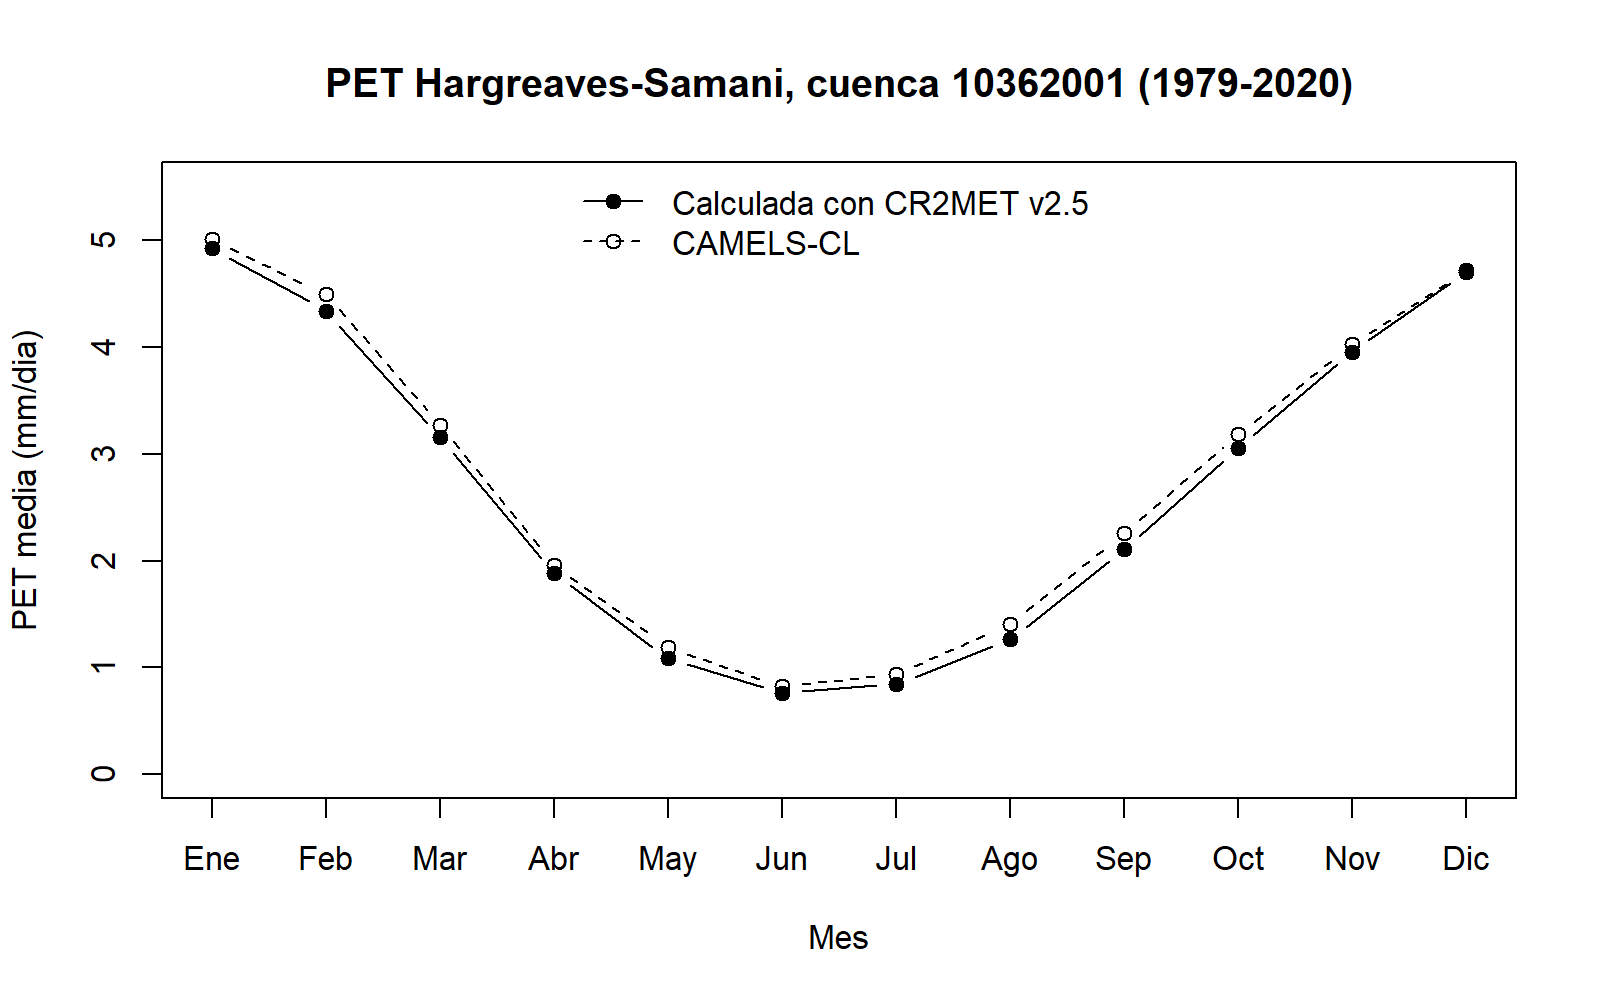
\includegraphics[width=0.8\textwidth]{../03_outputs/figures/04_PET_mensual_vs_CAMELS.png}}{%
\fbox{Falta 03\_outputs/figures/04\_PET\_mensual\_vs\_CAMELS.png}}
\caption{PET media de cada mes del año (mm\,día$^{-1}$), 1979-01 a 2020-04:
calculada con \citet{Hargreaves1985} sobre CR2MET v2.5 y la de CAMELS-CL
\citep{AlvarezGarreton2018}.}
\label{fig:E02pet}
\end{figure}

\campo{3. Fuente y trazabilidad}{Las grillas diarias de CR2MET v2.5 (0.05°,
WGS84) se promedian sobre el polígono de la cuenca delimitado en E01, ponderando cada celda por
la fracción que cae dentro, en \texttt{02\_\allowbreak{}Rscripts/\allowbreak{}04\_\allowbreak{}preparacion\_\allowbreak{}clima.R}.
El mismo script calcula la PET con la ecuación de \citet{Hargreaves1985} y la
radiación extraterrestre de \citet{Allen1998}, a la latitud del centroide del
polígono ($-$40.674°), y hace los controles día a día. La serie queda en
\texttt{01\_\allowbreak{}data/\allowbreak{}processed/\allowbreak{}clima\_\allowbreak{}CR2METv25\_\allowbreak{}10362001\_\allowbreak{}daily\_\allowbreak{}1960-2021.csv}.
El caudal es la serie diaria de la DGA rellenada por el integrante 2 en
\texttt{08b\_\allowbreak{}respaldo\_\allowbreak{}relleno\_\allowbreak{}Q.R} y \texttt{09\_\allowbreak{}consistencia\_\allowbreak{}Q.R}
(\texttt{01\_\allowbreak{}data/\allowbreak{}processed/\allowbreak{}caudal\_\allowbreak{}diario\_\allowbreak{}para\_\allowbreak{}airGR\_\allowbreak{}1987\_\allowbreak{}2019.csv}, que
trae juntas la columna observada, la completada y el método de cada día).
\texttt{02\_\allowbreak{}Rscripts/\allowbreak{}05\_\allowbreak{}regimen\_\allowbreak{}hidroclimatico.R} lo pasa a lámina con el
área del mismo polígono, cuenta los faltantes, aplica las pruebas de Pettitt,
ADF y KPSS (\texttt{05\_\allowbreak{}pettitt\_\allowbreak{}clima\_\allowbreak{}anual.csv} y
\texttt{05\_\allowbreak{}estacionariedad\_\allowbreak{}clima\_\allowbreak{}anual.csv}) y
escribe las cifras de esta ficha en
\texttt{03\_\allowbreak{}outputs/\allowbreak{}tables/\allowbreak{}05\_\allowbreak{}resumen\_\allowbreak{}calidad\_\allowbreak{}E02.csv}. Rutas, polígono y
período se leen de \texttt{06\_\allowbreak{}config/\allowbreak{}parametros.csv}, las fuentes del clima
están en \texttt{04\_\allowbreak{}metadata/\allowbreak{}data\_\allowbreak{}sources.csv} y todo se regenera con
\texttt{run\_\allowbreak{}all.R}.}

\campo{4. Interpretación hidrológica}{El clima no restringe el análisis:
CR2MET v2.5 cubre todos los días de 1960 a 2021 y pasa los controles. En P,
un cero es un día sin lluvia y no un dato faltante: CR2MET no trae NA, y los
controles los cuentan aparte. La variable que define qué años se pueden usar
es el caudal. Sus faltantes no son al azar: la mitad (174 de 347 días) cae
entre junio y agosto, cuando el caudal es mayor (máximo en julio y agosto,
E03). Un caudal anual calculado solo con los días disponibles quedaría bajo,
y descartar los años incompletos dejaría 22 de los 33. El equipo usa la serie
rellenada por el integrante 2: 5 días aislados por interpolación, febrero de
2009 con la mediana de ese mes y 12 bloques (314 días) por regresión con
estaciones vecinas, cada una elegida por validación cruzada. Así los 33 años
quedan completos y entra toda la información del período. El período termina
en 2019 porque 2020 tiene un 69.4 \% de días con caudal; 2021 está completo y
podría sumarse.

Budyko se aplica sobre promedios anuales, y para eso la P y la temperatura
tienen que ser homogéneas y estacionarias en el período que se usa. La prueba
de Pettitt responde si la mediana de una serie cambia en algún año. En
1987--2019 no detecta quiebre en P, PET ni Tmed: el menor $p$ es el de la
PET, 0.106. El KPSS no rechaza la estacionariedad en nivel en ninguna de las
tres ($p\geq$\,0.09; la PET queda cerca del 10 \%) y el ADF no rechaza la
raíz unitaria ($p$ entre 0.126 y 0.569). Las dos pruebas parten de hipótesis
nulas opuestas, aunque no exactamente complementarias: este ADF admite una
tendencia y el KPSS en nivel no. Ninguna muestra que las series dejen de ser
estacionarias, pero el ADF tampoco lo confirma.

En el registro completo sí hay cambios. Tmed sube unos 0.3 °C desde 1977, con
los dos valores $p$ bajo 0.05. La P baja 10 \% desde 1987, con $p=$\,0.043 en
la simulación; la aproximación da 0.059, así que ese quiebre queda en el borde
del 5 \%. El cambio de Tmed es anterior al período de análisis y el de P
coincide con su inicio, de modo que 1987--2019 queda entero después de los
dos. La PET sube 3.8 \% desde 2011 en el registro completo; dentro de
1987--2019 el cambio es de 2.9 \% y no resulta significativo. Las pruebas del
integrante 2 tampoco encuentran quiebre en el caudal anual rellenado.}

\campo{5. Consistencia física}{Los rangos de temperatura y de P diaria son
plausibles para una cuenca templada lluviosa del sur de Chile. Tmed queda
siempre entre Tmin y Tmax y el caudal observado nunca es cero ni negativo. La P de
CR2MET v2.5 difiere en 2.5 \% de la que trae CAMELS-CL (que no declara qué
versión de CR2MET usa), y la PET calculada en $-$3.8 \%, con correlaciones
diarias sobre 0.99. Mes a mes la PET difiere más en invierno, entre $-$7.6 y
$-$10.2 \% de mayo a agosto, cuando sus valores son menores. El orden de
magnitud coincide con el estudio nacional: la PET calculada
(973.4 mm\,año$^{-1}$) supera en 14.5 \% la isolínea de 850 y en 17.6 \% a
Cañal Bajo Osorno.}

\campo{6. Limitaciones e incertidumbre}{No se contrastó CR2MET con una
estación meteorológica dentro de la cuenca, así que la comparación entre
productos mide cuánto difieren, no cuál acierta. Tampoco se puede decir cuál
PET está más cerca de la real. \citet{Correa1997} usaron Penman con la
corrección de FAO-24, que según \citet{Allen1998} puede sobreestimar hasta un
20 \% con baja demanda evaporativa, y la ecuación de \citet{Hargreaves1985}
tiende a sobreestimar con humedad relativa alta \citep{Allen1998}. La PET usa
una sola latitud y se aplica a temperaturas ya promediadas en la cuenca. Con
33 años, un cambio chico como el de la PET dentro del período (2.9 \%) puede
no alcanzar a ser significativo. El ADF se corrió con 4 rezagos, como en la
clase práctica; con 33 años el valor por defecto del paquete sería 3. En 4
de los 12 bloques rellenados por regresión el error mediano de validación va
de 27.7 a 58.9 \%, sobre el 20 \% indicado en clase como límite defendible;
son bloques de verano y comienzos de otoño, con caudales bajos. En el bloque
del 17-12-2014 al 04-01-2015 la regresión dio valores negativos que quedaron
en 0 (19 días). Un caudal nulo no es físico en esta cuenca, cuyo mínimo
observado es 0.021 m$^3$\,s$^{-1}$.}

\campo{7. Conclusión asociada}{Entre 1987 y 2019 el caudal observado cubre el
97.1 \% de los días, pero solo 22 años están completos. Con el relleno del
integrante 2 los 33 años quedan completos y se pueden usar todos en el
balance y en el análisis de Budyko sobre promedios de largo plazo. El clima está completo y difiere menos de 4 \% de CAMELS-CL en
promedio anual. En ese período, P, PET y Tmed no muestran quiebres (Pettitt)
y el KPSS no rechaza su estacionariedad, aunque el ADF no la confirma.}

% Para que los pies digan "Tabla" y no "Cuadro", el preambulo del dossier
% debe decir \PassOptionsToPackage{spanish,es-tabla}{babel}.
% Cifras: 03_outputs/tables/05_resumen_calidad_E02.csv, 04_control_calidad_clima.csv,
% 04_PET_resumen_vs_CAMELS.csv, 04_PET_mensual_vs_CAMELS.csv, 05_pettitt_clima_anual.csv
% y 05_estacionariedad_clima_anual.csv,
% todas generadas por run_all.R.
% Periodo 1987-2019: acordado por el equipo el 19-oct (periodo_inicio y
% periodo_fin en 06_config).
% Fuente del caudal: Mapas DGA, reporte Caudal Diario Historico (fila Q_DGA de data_sources).
% Serie de caudal usada: la rellenada por Alexis (caudal_diario_para_airGR_1987_2019.csv),
% decidido por el equipo el 19-oct.
% Poligono: el de Alexis (cuenca_rio_damas.gpkg), desde el 19-oct.

\section{E02. Calidad y cobertura de la información}
\label{ev:E02}

\campo{1. Pregunta o afirmación que se evalúa}{¿Son suficientes y
consistentes la precipitación, las temperaturas, la PET y el caudal para
compararlos año a año en el período de análisis 1987--2019?}

\campo{2. Evidencia principal}{La Tabla~\ref{tab:E02cobertura} resume la
fuente, el registro y la cobertura de cada variable, y la
Figura~\ref{fig:E02faltantes} muestra dónde están los días sin caudal. La
Tabla~\ref{tab:E02controles} reúne los controles y las comparaciones con
otras fuentes. Las Tablas~\ref{tab:E02pettitt} y~\ref{tab:E02estacionariedad}
muestran las pruebas de homogeneidad y estacionariedad de las series anuales
del clima. La Figura~\ref{fig:E02pet} compara el ciclo
anual de la PET calculada con el de CAMELS-CL.}

\begin{table}[ht]
\centering
\caption{Fuente, registro y cobertura por variable. Cobertura: porcentaje de
días con dato dentro de 1987--2019.}
\label{tab:E02cobertura}
\begin{tabular}{|p{0.17\linewidth}|p{0.32\linewidth}|p{0.17\linewidth}|p{0.16\linewidth}|}
\hline
Variable (unidad) & Fuente & Registro & Cobertura 1987--2019, en \% \\
\hline
P (mm\,día$^{-1}$) & CR2MET v2.5 \citep{Boisier2023} & 1960-01-01 a 2021-12-31 & 100 \\
\hline
Tmax, Tmin (°C) & CR2MET v2.5 \citep{Boisier2023} & 1960-01-01 a 2021-12-31 & 100 \\
\hline
Tmed (°C) & (Tmax + Tmin)/2 & 1960-01-01 a 2021-12-31 & 100 \\
\hline
PET (mm\,día$^{-1}$) & \citet{Hargreaves1985} con Tmax y Tmin de CR2MET v2.5 & 1960-01-01 a 2021-12-31 & 100 \\
\hline
Q (m$^3$\,s$^{-1}$) & DGA, estación Río Damas en Tacamo \citep{DGA_mapas}, rellenada por el integrante 2 & 1986-02-01 a 2026-06-15 & 97.12 observado (347 días sin dato); 100 con el relleno \\
\hline
\end{tabular}
\end{table}

\begin{figure}[ht]
\centering
\IfFileExists{../03_outputs/figures/05_cobertura_caudal.png}{%
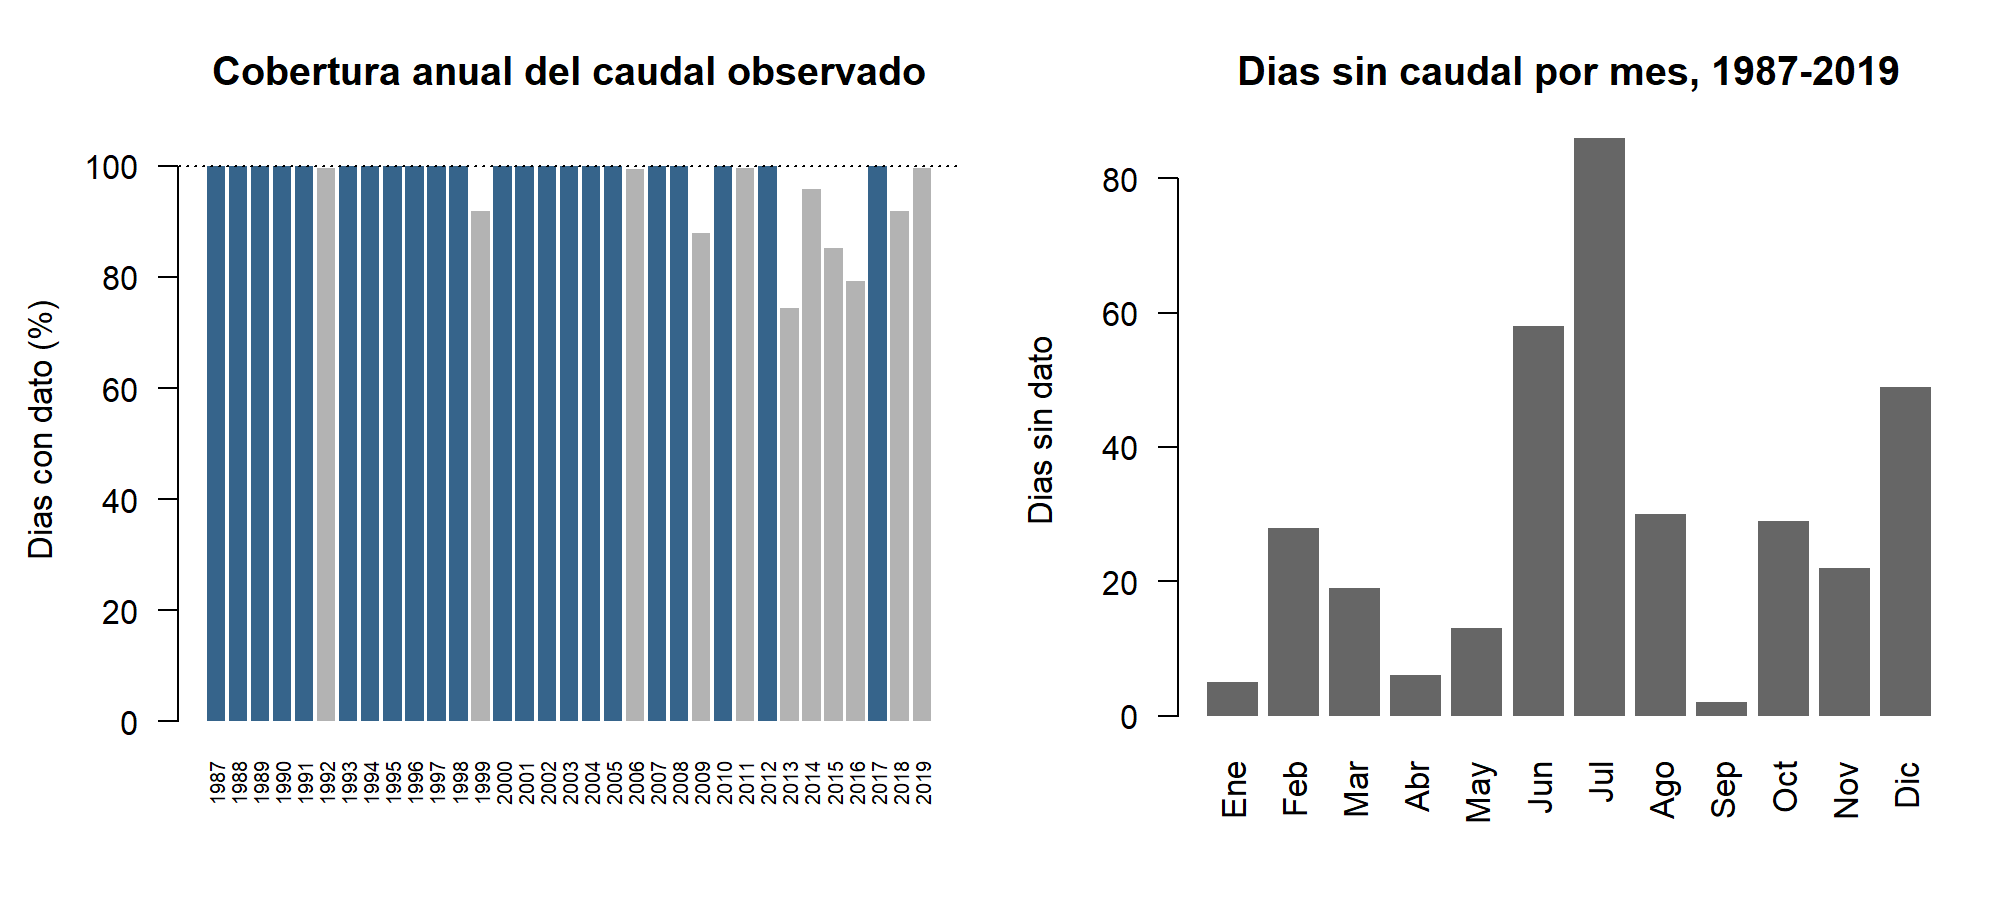
\includegraphics[width=0.95\textwidth]{../03_outputs/figures/05_cobertura_caudal.png}}{%
\fbox{Falta 03\_outputs/figures/05\_cobertura\_caudal.png}}
\caption{Faltantes del caudal DGA observado, antes del relleno. Izquierda:
porcentaje de días con dato en cada año calendario de 1987--2019 (gris: año
incompleto). Derecha: días sin dato por mes del año, sumados en 1987--2019.}
\label{fig:E02faltantes}
\end{figure}

\begin{table}[ht]
\centering
\caption{Controles de calidad y comparación entre fuentes.}
\label{tab:E02controles}
\begin{tabular}{|p{0.42\linewidth}|p{0.16\linewidth}|p{0.27\linewidth}|}
\hline
Control & Período & Resultado \\
\hline
Fechas duplicadas, días faltantes y NA en P, Tmax, Tmin y PET & 1960--2021 & 0 de 22646 días \\
\hline
P negativa, Tmin mayor que Tmax, Tmed fuera de [Tmin, Tmax], PET negativa & 1960--2021 & 0 días \\
\hline
Tmax y Tmin diarias & 1987--2019 & 4.0 a 36.9 °C y $-$6.3 a 16.5 °C \\
\hline
P diaria máxima & 1987--2019 & 85.6 mm\,día$^{-1}$ (2004-04-02) \\
\hline
PET diaria & 1987--2019 & 0.43 a 7.91 mm\,día$^{-1}$ \\
\hline
Q observado diario & 1987--2019 & 0.021 a 157 m$^3$\,s$^{-1}$, sin valores $\le$\,0 \\
\hline
Días sin Q en junio, julio y agosto & 1987--2019 & 174 de 347 \\
\hline
Años calendario con Q observado completo & 1987--2019 & 22 de 33 \\
\hline
Días rellenados por el integrante 2 & 1987--2019 & 314 por regresión con estaciones vecinas (12 bloques), 28 con la mediana de febrero (2009) y 5 por interpolación \\
\hline
Bloques por regresión con error mediano de validación bajo 20 \% & 1987--2019 & 8 de 12; los otros 4, entre 27.7 y 58.9 \% \\
\hline
Días con Q rellenado igual a 0 & 2014-12-17 a 2015-01-04 & 19 \\
\hline
Años calendario con Q completo tras el relleno & 1987--2019 & 33 de 33 \\
\hline
Homogeneidad del Q anual rellenado (integrante 2) & 1987--2019 & sin quiebre: Pettitt $p=$\,0.99, Buishand $p=$\,0.70, SNHT $p=$\,0.27 \\
\hline
P media anual de los 33 años & 1987--2019 & 1601.6 mm\,año$^{-1}$ \\
\hline
P de CR2MET v2.5 frente a la de CAMELS-CL \citep{AlvarezGarreton2018} & 1979-01 a 2020-04 & 1633.9 y 1594.1 mm\,año$^{-1}$ (+2.5 \%); $r=$\,0.992 \\
\hline
PET calculada frente a la de CAMELS-CL & 1979-01 a 2020-04 & 974.3 y 1013.2 mm\,año$^{-1}$ ($-$3.8 \%); $r=$\,0.994 \\
\hline
PET media anual calculada & 1987--2019 & 973.4 mm\,año$^{-1}$ \\
\hline
PET anual en la lámina 12 de \citet{Correa1997} & registros hasta 1991 & sobre 850 mm\,año$^{-1}$ al oeste, cerca de 800 al este \\
\hline
PET anual de las estaciones de \citet{Correa1997} en los bordes de la cuenca & registros hasta 1991 & 827.5 (Cañal Bajo Osorno, oeste) y 701.9 mm\,año$^{-1}$ (Central Pilmaiquén, este) \\
\hline
\end{tabular}
\end{table}

\begin{table}[ht]
\centering
\caption{Prueba de Pettitt \citep{Pettitt1979} sobre las series anuales del
clima, en el período de análisis (1987--2019, 33 años) y en el registro
completo (1960--2021, 62 años). Hipótesis nula: no hay cambio en la mediana
de la serie; la prueba trabaja con los signos de las diferencias entre años,
no con los valores. Nivel de significancia: 5 \%. $p$ por simulación: 999
permutaciones, como en la clase práctica CP05. $p$ aproximado: fórmula
asintótica de \citet{Pettitt1979}, solo como referencia y acotada a 1. Las
medias antes y después del año de quiebre describen el tamaño del cambio.}
\label{tab:E02pettitt}
\begin{tabular}{|p{0.17\linewidth}|p{0.1\linewidth}|p{0.13\linewidth}|p{0.11\linewidth}|p{0.11\linewidth}|p{0.1\linewidth}|p{0.1\linewidth}|}
\hline
Variable & Tramo & Último año\newline antes del\newline quiebre & $p$\newline simulación & $p$\newline aproximado & Media\newline antes & Media\newline después \\
\hline
P (mm\,año$^{-1}$) & 1987--2019 & 1991 & 0.865 & 1 & 1484.1 & 1622.6 \\
\hline
PET (mm\,año$^{-1}$) & 1987--2019 & 2010 & 0.106 & 0.141 & 965.7 & 993.6 \\
\hline
Tmed (°C) & 1987--2019 & 2012 & 0.396 & 0.538 & 11.22 & 11.48 \\
\hline
P (mm\,año$^{-1}$) & 1960--2021 & 1986 & 0.043 & 0.059 & 1761.2 & 1578.7 \\
\hline
PET (mm\,año$^{-1}$) & 1960--2021 & 2010 & 0.026 & 0.047 & 961.1 & 997.4 \\
\hline
Tmed (°C) & 1960--2021 & 1976 & 0.020 & 0.025 & 10.97 & 11.30 \\
\hline
\end{tabular}
\end{table}

\begin{table}[ht]
\centering
\caption{Estacionariedad de las series anuales del clima en 1987--2019 (33
años), con las mismas llamadas de la clase práctica CP05 en el paquete
tseries \citep{tseries}. ADF \citep{SaidDickey1984}: hipótesis nula de raíz
unitaria (serie no estacionaria); incluye intercepto y tendencia, con 4
rezagos. KPSS \citep{Kwiatkowski1992}: hipótesis nula de estacionariedad en
nivel. Nivel de significancia: 5 \%. El paquete acota el $p$ del KPSS a 0.1,
así que 0.1 significa 0.1 o más.}
\label{tab:E02estacionariedad}
\begin{tabular}{|p{0.2\linewidth}|p{0.15\linewidth}|p{0.1\linewidth}|p{0.15\linewidth}|p{0.1\linewidth}|}
\hline
Variable & ADF,\newline estadístico & ADF, $p$ & KPSS,\newline estadístico & KPSS, $p$ \\
\hline
P (mm\,año$^{-1}$) & $-$3.157 & 0.126 & 0.086 & 0.1 \\
\hline
PET (mm\,año$^{-1}$) & $-$2.465 & 0.393 & 0.362 & 0.094 \\
\hline
Tmed (°C) & $-$2.011 & 0.569 & 0.112 & 0.1 \\
\hline
\end{tabular}
\end{table}

\begin{figure}[ht]
\centering
\IfFileExists{../03_outputs/figures/04_PET_mensual_vs_CAMELS.png}{%
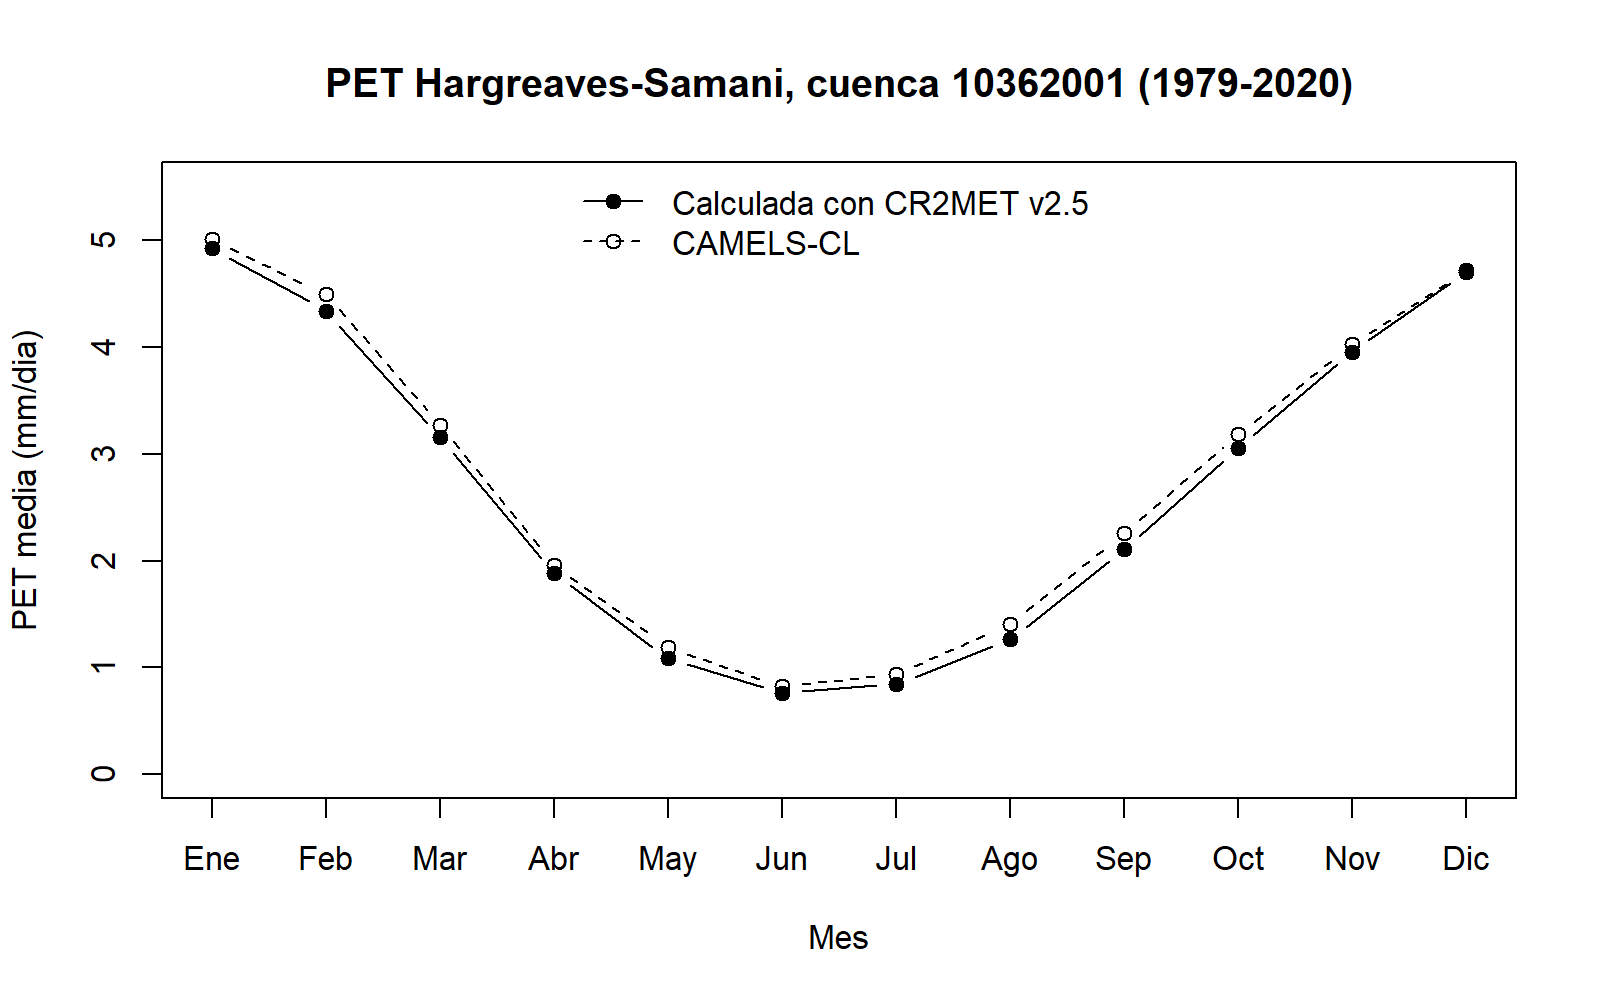
\includegraphics[width=0.8\textwidth]{../03_outputs/figures/04_PET_mensual_vs_CAMELS.png}}{%
\fbox{Falta 03\_outputs/figures/04\_PET\_mensual\_vs\_CAMELS.png}}
\caption{PET media de cada mes del año (mm\,día$^{-1}$), 1979-01 a 2020-04:
calculada con \citet{Hargreaves1985} sobre CR2MET v2.5 y la de CAMELS-CL
\citep{AlvarezGarreton2018}.}
\label{fig:E02pet}
\end{figure}

\campo{3. Fuente y trazabilidad}{Las grillas diarias de CR2MET v2.5 (0.05°,
WGS84) se promedian sobre el polígono de la cuenca delimitado en E01, ponderando cada celda por
la fracción que cae dentro, en \texttt{02\_\allowbreak{}Rscripts/\allowbreak{}04\_\allowbreak{}preparacion\_\allowbreak{}clima.R}.
El mismo script calcula la PET con la ecuación de \citet{Hargreaves1985} y la
radiación extraterrestre de \citet{Allen1998}, a la latitud del centroide del
polígono ($-$40.674°), y hace los controles día a día. La serie queda en
\texttt{01\_\allowbreak{}data/\allowbreak{}processed/\allowbreak{}clima\_\allowbreak{}CR2METv25\_\allowbreak{}10362001\_\allowbreak{}daily\_\allowbreak{}1960-2021.csv}.
El caudal es la serie diaria de la DGA rellenada por el integrante 2 en
\texttt{08b\_\allowbreak{}respaldo\_\allowbreak{}relleno\_\allowbreak{}Q.R} y \texttt{09\_\allowbreak{}consistencia\_\allowbreak{}Q.R}
(\texttt{01\_\allowbreak{}data/\allowbreak{}processed/\allowbreak{}caudal\_\allowbreak{}diario\_\allowbreak{}para\_\allowbreak{}airGR\_\allowbreak{}1987\_\allowbreak{}2019.csv}, que
trae juntas la columna observada, la completada y el método de cada día).
\texttt{02\_\allowbreak{}Rscripts/\allowbreak{}05\_\allowbreak{}regimen\_\allowbreak{}hidroclimatico.R} lo pasa a lámina con el
área del mismo polígono, cuenta los faltantes, aplica las pruebas de Pettitt,
ADF y KPSS (\texttt{05\_\allowbreak{}pettitt\_\allowbreak{}clima\_\allowbreak{}anual.csv} y
\texttt{05\_\allowbreak{}estacionariedad\_\allowbreak{}clima\_\allowbreak{}anual.csv}) y
escribe las cifras de esta ficha en
\texttt{03\_\allowbreak{}outputs/\allowbreak{}tables/\allowbreak{}05\_\allowbreak{}resumen\_\allowbreak{}calidad\_\allowbreak{}E02.csv}. Rutas, polígono y
período se leen de \texttt{06\_\allowbreak{}config/\allowbreak{}parametros.csv}, las fuentes del clima
están en \texttt{04\_\allowbreak{}metadata/\allowbreak{}data\_\allowbreak{}sources.csv} y todo se regenera con
\texttt{run\_\allowbreak{}all.R}.}

\campo{4. Interpretación hidrológica}{El clima no restringe el análisis:
CR2MET v2.5 cubre todos los días de 1960 a 2021 y pasa los controles. En P,
un cero es un día sin lluvia y no un dato faltante: CR2MET no trae NA, y los
controles los cuentan aparte. La variable que define qué años se pueden usar
es el caudal. Sus faltantes no son al azar: la mitad (174 de 347 días) cae
entre junio y agosto, cuando el caudal es mayor (máximo en julio y agosto,
E03). Un caudal anual calculado solo con los días disponibles quedaría bajo,
y descartar los años incompletos dejaría 22 de los 33. El equipo usa la serie
rellenada por el integrante 2: 5 días aislados por interpolación, febrero de
2009 con la mediana de ese mes y 12 bloques (314 días) por regresión con
estaciones vecinas, cada una elegida por validación cruzada. Así los 33 años
quedan completos y entra toda la información del período. El período termina
en 2019 porque 2020 tiene un 69.4 \% de días con caudal; 2021 está completo y
podría sumarse.

Budyko se aplica sobre promedios anuales, y para eso la P y la temperatura
tienen que ser homogéneas y estacionarias en el período que se usa. La prueba
de Pettitt responde si la mediana de una serie cambia en algún año. En
1987--2019 no detecta quiebre en P, PET ni Tmed: el menor $p$ es el de la
PET, 0.106. El KPSS no rechaza la estacionariedad en nivel en ninguna de las
tres ($p\geq$\,0.09; la PET queda cerca del 10 \%) y el ADF no rechaza la
raíz unitaria ($p$ entre 0.126 y 0.569). Las dos pruebas parten de hipótesis
nulas opuestas, aunque no exactamente complementarias: este ADF admite una
tendencia y el KPSS en nivel no. Ninguna muestra que las series dejen de ser
estacionarias, pero el ADF tampoco lo confirma.

En el registro completo sí hay cambios. Tmed sube unos 0.3 °C desde 1977, con
los dos valores $p$ bajo 0.05. La P baja 10 \% desde 1987, con $p=$\,0.043 en
la simulación; la aproximación da 0.059, así que ese quiebre queda en el borde
del 5 \%. El cambio de Tmed es anterior al período de análisis y el de P
coincide con su inicio, de modo que 1987--2019 queda entero después de los
dos. La PET sube 3.8 \% desde 2011 en el registro completo; dentro de
1987--2019 el cambio es de 2.9 \% y no resulta significativo. Las pruebas del
integrante 2 tampoco encuentran quiebre en el caudal anual rellenado.}

\campo{5. Consistencia física}{Los rangos de temperatura y de P diaria son
plausibles para una cuenca templada lluviosa del sur de Chile. Tmed queda
siempre entre Tmin y Tmax y el caudal observado nunca es cero ni negativo. La P de
CR2MET v2.5 difiere en 2.5 \% de la que trae CAMELS-CL (que no declara qué
versión de CR2MET usa), y la PET calculada en $-$3.8 \%, con correlaciones
diarias sobre 0.99. Mes a mes la PET difiere más en invierno, entre $-$7.6 y
$-$10.2 \% de mayo a agosto, cuando sus valores son menores. El orden de
magnitud coincide con el estudio nacional: la PET calculada
(973.4 mm\,año$^{-1}$) supera en 14.5 \% la isolínea de 850 y en 17.6 \% a
Cañal Bajo Osorno.}

\campo{6. Limitaciones e incertidumbre}{No se contrastó CR2MET con una
estación meteorológica dentro de la cuenca, así que la comparación entre
productos mide cuánto difieren, no cuál acierta. Tampoco se puede decir cuál
PET está más cerca de la real. \citet{Correa1997} usaron Penman con la
corrección de FAO-24, que según \citet{Allen1998} puede sobreestimar hasta un
20 \% con baja demanda evaporativa, y la ecuación de \citet{Hargreaves1985}
tiende a sobreestimar con humedad relativa alta \citep{Allen1998}. La PET usa
una sola latitud y se aplica a temperaturas ya promediadas en la cuenca. Con
33 años, un cambio chico como el de la PET dentro del período (2.9 \%) puede
no alcanzar a ser significativo. El ADF se corrió con 4 rezagos, como en la
clase práctica; con 33 años el valor por defecto del paquete sería 3. En 4
de los 12 bloques rellenados por regresión el error mediano de validación va
de 27.7 a 58.9 \%, sobre el 20 \% indicado en clase como límite defendible;
son bloques de verano y comienzos de otoño, con caudales bajos. En el bloque
del 17-12-2014 al 04-01-2015 la regresión dio valores negativos que quedaron
en 0 (19 días). Un caudal nulo no es físico en esta cuenca, cuyo mínimo
observado es 0.021 m$^3$\,s$^{-1}$.}

\campo{7. Conclusión asociada}{Entre 1987 y 2019 el caudal observado cubre el
97.1 \% de los días, pero solo 22 años están completos. Con el relleno del
integrante 2 los 33 años quedan completos y se pueden usar todos en el
balance y en el análisis de Budyko sobre promedios de largo plazo. El clima está completo y difiere menos de 4 \% de CAMELS-CL en
promedio anual. En ese período, P, PET y Tmed no muestran quiebres (Pettitt)
y el KPSS no rechaza su estacionariedad, aunque el ADF no la confirma.}
